%
% $RCSfile: paradigm_and_language.tex,v $
%
% Copyright (C) 2002-2008. Christian Heller.
%
% Permission is granted to copy, distribute and/or modify this document
% under the terms of the GNU Free Documentation License, Version 1.1 or
% any later version published by the Free Software Foundation; with no
% Invariant Sections, with no Front-Cover Texts and with no Back-Cover
% Texts. A copy of the license is included in the section entitled
% "GNU Free Documentation License".
%
% http://www.cybop.net
% - Cybernetics Oriented Programming -
%
% http://www.resmedicinae.org
% - Information in Medicine -
%
% Version: $Revision: 1.1 $ $Date: 2008-08-19 20:41:08 $ $Author: christian $
% Authors: Christian Heller <christian.heller@tuxtax.de>
%

\section{Paradigm and Language}
\label{paradigm_and_language_heading}
\index{Paradigm and Language}
\index{Computer Language}
\index{Programming Language}
\index{Markup Language}
\index{Data Manipulation Language}
\index{DML}
\index{Page Description Language}
\index{Specification Language}

Manifold instructions exist that allow humans to program a computer. A set of
such instructions is called \emph{Programming Language} and is one of many
groups of different \emph{Computer Languages}. Other groups are for example
\emph{Markup Languages}, \emph{Data Manipulation Languages} (DML),
\emph{Page Description Languages} or \emph{Specification Languages}
\cite{wikipedia}.

%
% $RCSfile: language_history.tex,v $
%
% Copyright (C) 2002-2008. Christian Heller.
%
% Permission is granted to copy, distribute and/or modify this document
% under the terms of the GNU Free Documentation License, Version 1.1 or
% any later version published by the Free Software Foundation; with no
% Invariant Sections, with no Front-Cover Texts and with no Back-Cover
% Texts. A copy of the license is included in the section entitled
% "GNU Free Documentation License".
%
% http://www.cybop.net
% - Cybernetics Oriented Programming -
%
% http://www.resmedicinae.org
% - Information in Medicine -
%
% Version: $Revision: 1.1 $ $Date: 2008-08-19 20:41:07 $ $Author: christian $
% Authors: Christian Heller <christian.heller@tuxtax.de>
%

\subsection{Language History}
\label{language_history_heading}
\index{Language History}
\index{Programming Paradigm}
\index{Computer Languages Timeline}
\index{Language List}
\index{Programming Language Generations}

Just as a software engineering school advocates its very own \emph{Methodology}
(chapter \ref{software_engineering_process_heading}), each programming language
advocates a special \emph{Programming Paradigm} \cite{wikipedia} (sometimes
also more than one). Some efforts categorise languages or their paradigms
historically \cite{steppan}. Eric Levenez' \emph{Computer Languages Timeline}
\cite{levenez} captures common programming languages from a historical
perspective. Some of them are shown in the simplified figure
\ref{language_figure} (whose columns have no meaning). A much more
comprehensive overview listing more than 2500 languages is given in the
\emph{Language List} \cite{kinnersley} of Bill Kinnersley.

\begin{figure}[ht]
    \begin{center}
        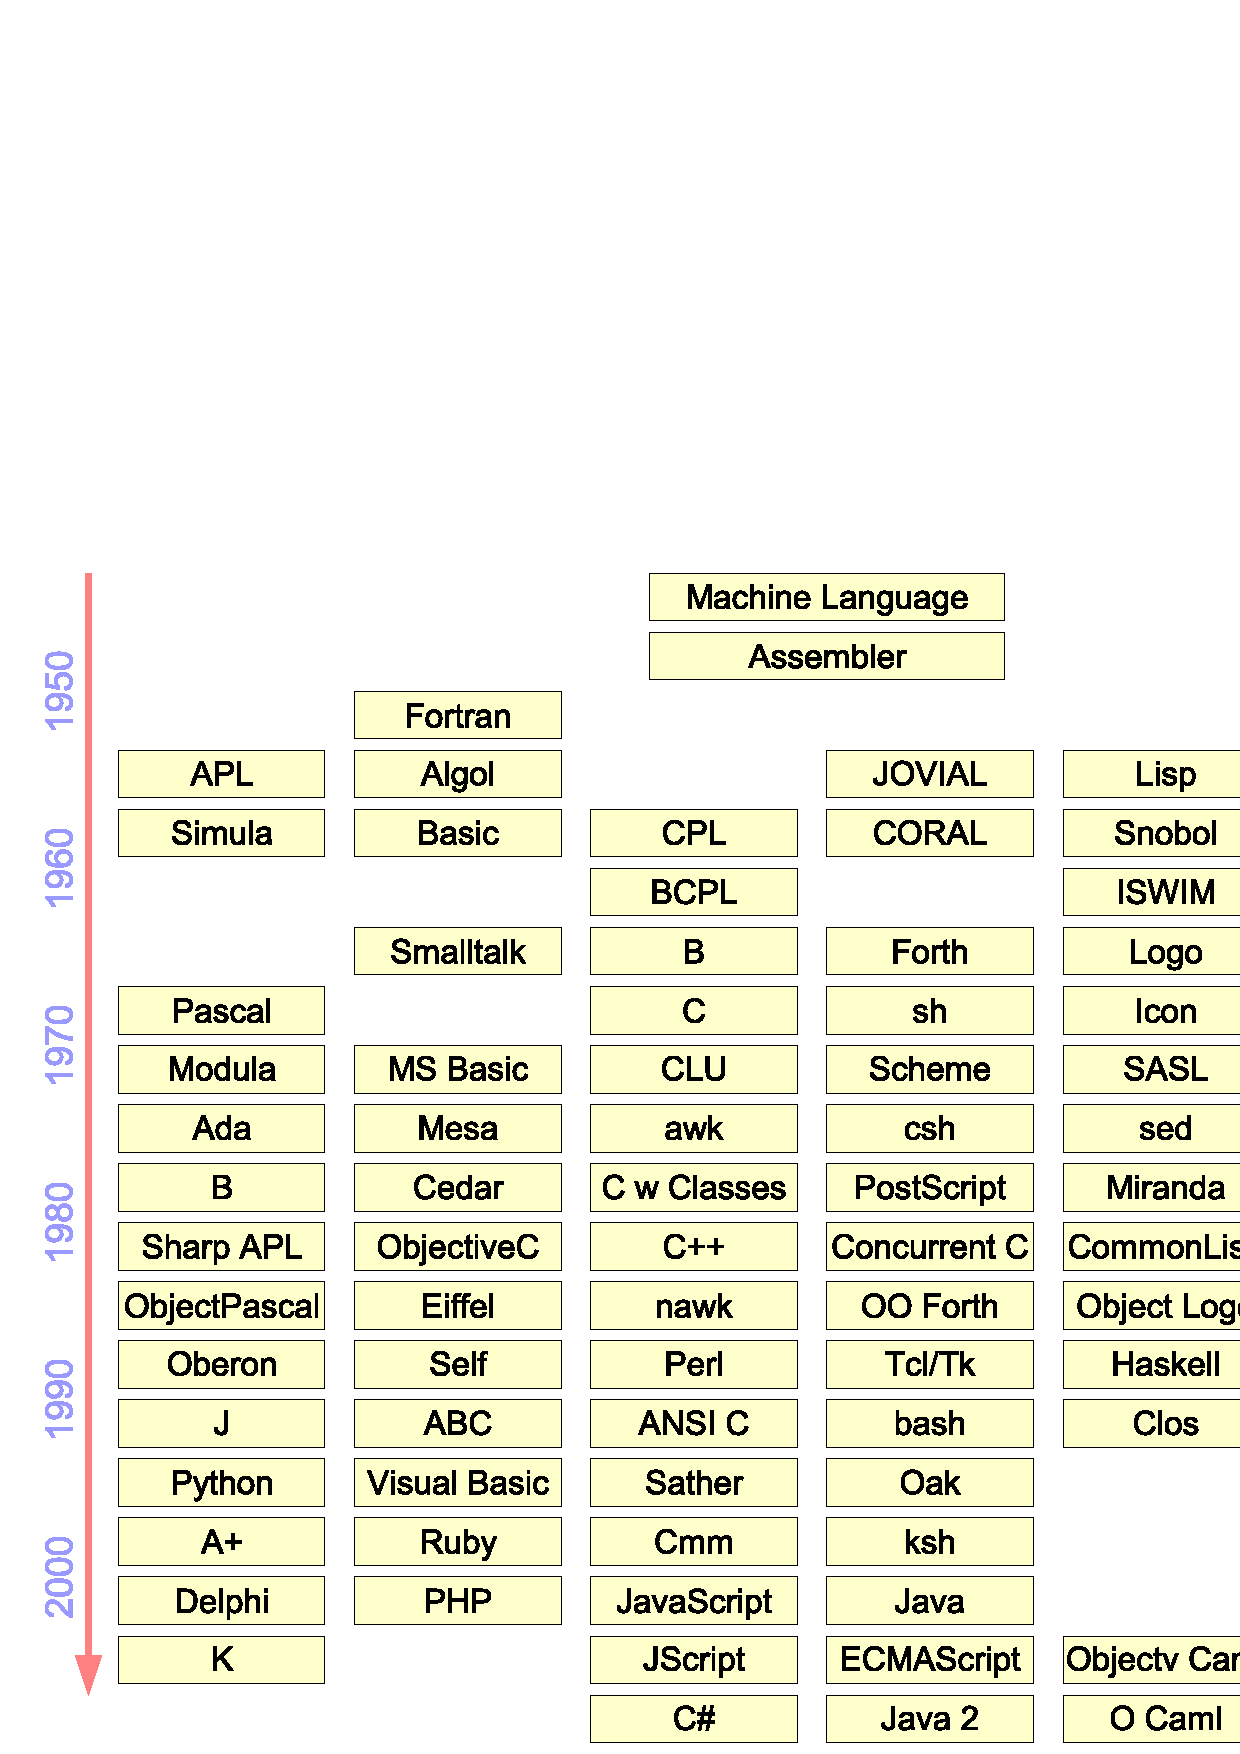
\includegraphics[scale=0.3,angle=-90]{graphic/language.pdf}
        \caption{Programming Language History}
        \label{language_figure}
    \end{center}
\end{figure}

A lineage can be identified for every language, some popular of which are shown
in the following list, the corresponding language name mentioned at first,
being followed by the names of the language's ancestors. The right-most
language represents the oldest ancestor. Only \emph{one} lineage of arbitrary
choice is considered for each language; most languages have \emph{further}
ancestors that are not mentioned here:

\begin{itemize}
    \item[-] \emph{Java 2:} Java 1, Oak, Cedar, Mesa, Algol, IAL, Fortran
    \item[-] \emph{C\#:} C++, C with Classes, C, B, BCPL, CPL, Algol
    \item[-] \emph{VB.NET:} Visual Basic, MS Basic, Basic, Algol
    \item[-] \emph{Delphi:} Object Pascal, Pascal, Algol
    \item[-] \emph{Oberon:} Modula, Pascal
    \item[-] \emph{Self:} Smalltalk, Simula, Algol
    \item[-] \emph{Tcl/Tk:} Tcl
    \item[-] \emph{Python:} ABC, B
    \item[-] \emph{Perl:} nawk, awk, Icon, Snobol
    \item[-] \emph{PHP:} PHP/FI, Perl
    \item[-] \emph{Ruby:} CLU, Pascal
    \item[-] \emph{Haskell:} Miranda, KRC, SASL, ISWIM
    \item[-] \emph{O Caml:} Objective Caml, Caml, SML, ML
    \item[-] \emph{OO COBOL:} COBOL, Flow-Matic, B-O
    \item[-] \emph{NetRexx:} Object Rexx, Rexx, Rex, PL/1 ANS, PL/M, PL/I, COBOL
    \item[-] \emph{Open M:} M, MUMPS
    \item[-] \emph{Scheme:} Common Lisp, Lisp
    \item[-] \emph{PostScript:} OO Forth, Forth
\end{itemize}

Other historical approaches assign each programming language to a special
\emph{Generation}. Commonly used programming language generations and some of
their representatives are shown following \cite{wikipedia}:

\begin{itemize}
    \item[-] \emph{First Generation Language}: machine-level language
    \item[-] \emph{Second Generation Language}: assembly language
    \item[-] \emph{Third Generation Language} (3GL): Fortran, Algol, COBOL, Basic, C, C++
    \item[-] \emph{Fourth Generation Language} (4GL): SQL, Mathematica, SAS, VB, MATLAB
    \item[-] \emph{Fifth Generation Language}: Prolog, OPS5, Mercury
\end{itemize}

%
% $RCSfile: paradigm_overview.tex,v $
%
% Copyright (C) 2002-2008. Christian Heller.
%
% Permission is granted to copy, distribute and/or modify this document
% under the terms of the GNU Free Documentation License, Version 1.1 or
% any later version published by the Free Software Foundation; with no
% Invariant Sections, with no Front-Cover Texts and with no Back-Cover
% Texts. A copy of the license is included in the section entitled
% "GNU Free Documentation License".
%
% http://www.cybop.net
% - Cybernetics Oriented Programming -
%
% http://www.resmedicinae.org
% - Information in Medicine -
%
% Version: $Revision: 1.1 $ $Date: 2008-08-19 20:41:08 $ $Author: christian $
% Authors: Christian Heller <christian.heller@tuxtax.de>
%

\subsection{Paradigm Overview}
\label{paradigm_overview_heading}
\index{Paradigm Overview}
\index{Programming Paradigm Systematics}
\index{Imperative (Command Oriented) Programming Language}
\index{Declarative Programming Language}
\index{Machine Language}
\index{Assembly Language}
\index{System Programming}
\index{Functional Programming}
\index{Logical Programming}
\index{Scripting Language}
\index{Typeless Programming}
\index{Structured- and Procedural Programming}
\index{SPP}
\index{Object Oriented Programming}
\index{OOP}
\index{Programming Paradigms as Contrasting Pairs}

Several other systematics, besides the historical one shown in the previous
section, exist to categorise programming languages and their paradigms. Some
authors, for example, divide computer languages into those that have to be
compiled before being executed and those which are interpreted at runtime.
Figure \ref{paradigm_figure} shows yet another arbitrary, tree-like systematics
that was assembled on the basis of \cite{wikipedia} and \cite{kinnersley}.

\begin{figure}[ht]
    \begin{center}
        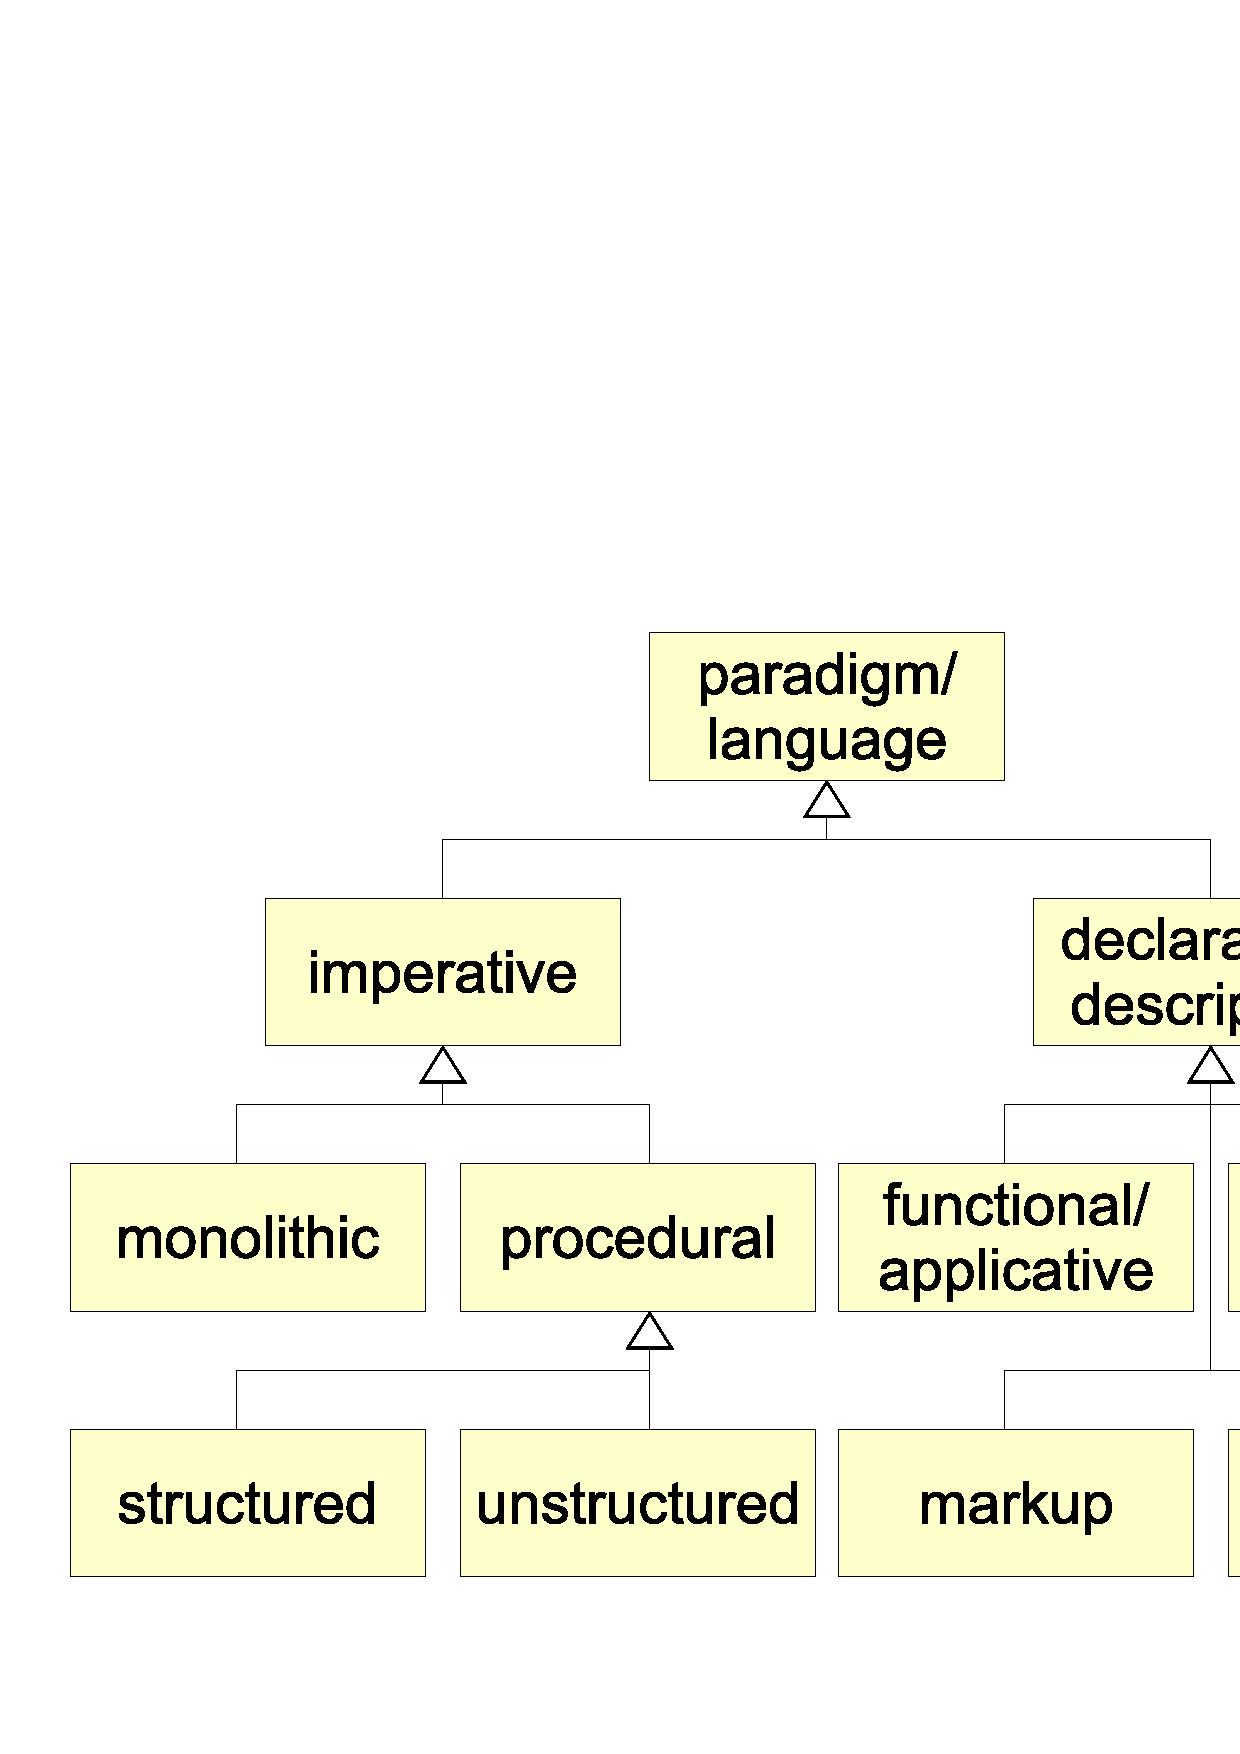
\includegraphics[scale=0.3,angle=-90]{graphic/paradigm.pdf}
        \caption{Programming Paradigm Systematics}
        \label{paradigm_figure}
    \end{center}
\end{figure}

\emph{Machine-} and \emph{Assembly Language} as well as \emph{System Programming}
are \emph{imperative} (command-oriented). \emph{Functional-} and
\emph{Logical Programming}, on the other hand, are \emph{declarative}, just as
most \emph{Scripting Languages} used for \emph{Typeless Programming}. The
boundaries tend to be vague, however. Many of the new languages borrow features
from more than one programming paradigm. Similarly, the concepts of
\emph{Structured and Procedural Programming} (SPP) and
\emph{Object Oriented Programming} (OOP) are not only used in system
programming-, but also in scripting languages.

It is important to note that it is extremely difficult, if not impossible, to
arrange all programming languages into just one tree of categories. Kinnersley
\cite{kinnersley} writes that \textit{for every classification scheme there
will be a large proportion of languages that do not fit \ldots\ most languages
are not purely one or the other}. The \emph{Logo} language, for example, is an
adaptation of the functional language \emph{Lisp}, that is non-imperative, yet
procedural \cite{wikipedia}. Figure \ref{paradigm_figure} can therefore only be
seen as trial to create a systematics of the most common programming paradigms.
In order to avoid miscategorisation, the Wikipedia Encyclopedia \cite{wikipedia}
prefers to list programming paradigms as contrasting pairs, for example:

\begin{itemize}
    \item[-] Procedural vs. Functional
    \item[-] Imperative vs. Declarative
    \item[-] Structured vs. Unstructured
    \item[-] Value-level vs. Function-level
    \item[-] Flow-driven vs. Event-driven
    \item[-] Scalar vs. Array
    \item[-] Class-based vs. Prototype-based
    \item[-] Rule-based vs. Constraint
\end{itemize}

Not all items of the list are explained in this work since this would break its
frame and focus. However, some of the most important programming language
concepts in use today are described in the following sections.

%
% $RCSfile: hardware_architecture.tex,v $
%
% Copyright (C) 2002-2008. Christian Heller.
%
% Permission is granted to copy, distribute and/or modify this document
% under the terms of the GNU Free Documentation License, Version 1.1 or
% any later version published by the Free Software Foundation; with no
% Invariant Sections, with no Front-Cover Texts and with no Back-Cover
% Texts. A copy of the license is included in the section entitled
% "GNU Free Documentation License".
%
% http://www.cybop.net
% - Cybernetics Oriented Programming -
%
% http://www.resmedicinae.org
% - Information in Medicine -
%
% Version: $Revision: 1.1 $ $Date: 2008-08-19 20:41:07 $ $Author: christian $
% Authors: Christian Heller <christian.heller@tuxtax.de>
%

\subsection{Hardware Architecture}
\label{hardware_architecture_heading}
\index{Hardware Architecture}
\index{Abstract Levels of a Virtual Machine}
\index{Virtual Machine}
\index{VM}
\index{Computer Structure}
\index{Lower Levels of a Computer Structure}
\index{Higher Levels of a Computer Structure}
\index{Problem Oriented Languages}
\index{POL}

In his very clear book, Tanenbaum \cite{tanenbaum1999} organises instructions
in abstract \emph{Levels} (figure \ref{vm_figure}), which he also calls
\emph{Virtual Machines} (VM), since each level could be seen as hypothetic
computer with an own language. Further on, he considers hardware and software
to be \textit{logically equivalent} because one could replace the other.

\begin{figure}[ht]
    \begin{center}
        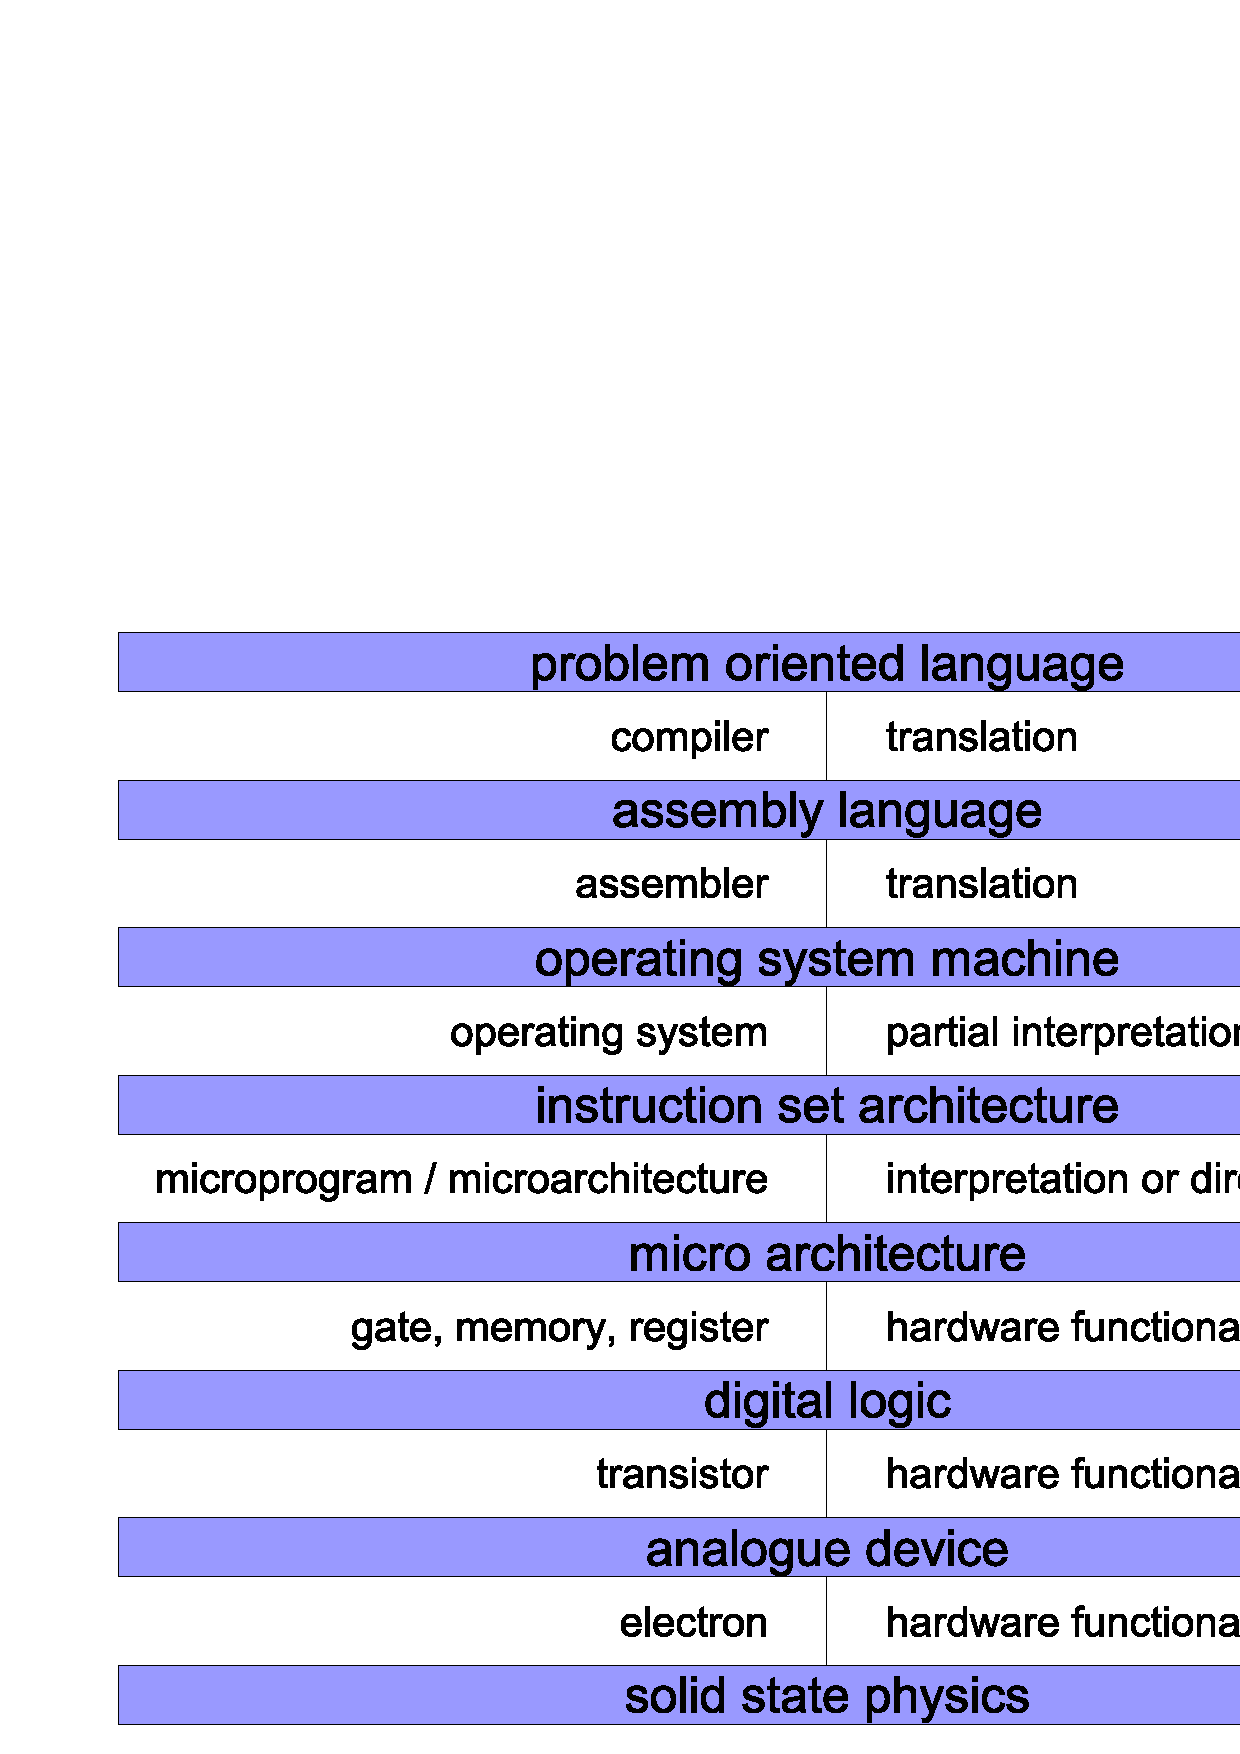
\includegraphics[scale=0.3,angle=-90]{graphic/vm.pdf}
        \caption{Computer Structure (adapted from \cite{tanenbaum1999})}
        \label{vm_figure}
    \end{center}
\end{figure}

The next sub sections are based on this structure. They describe lower levels,
close to hardware. Later sections then place more emphasis on concepts
introduced by higher-level \emph{Problem Oriented Languages} (POL).

%
% $RCSfile: digital_logic.tex,v $
%
% Copyright (C) 2002-2008. Christian Heller.
%
% Permission is granted to copy, distribute and/or modify this document
% under the terms of the GNU Free Documentation License, Version 1.1 or
% any later version published by the Free Software Foundation; with no
% Invariant Sections, with no Front-Cover Texts and with no Back-Cover
% Texts. A copy of the license is included in the section entitled
% "GNU Free Documentation License".
%
% http://www.cybop.net
% - Cybernetics Oriented Programming -
%
% http://www.resmedicinae.org
% - Information in Medicine -
%
% Version: $Revision: 1.1 $ $Date: 2008-08-19 20:41:06 $ $Author: christian $
% Authors: Christian Heller <christian.heller@tuxtax.de>
%

\subsubsection{Digital Logic}
\label{digital_logic_heading}
\index{Digital Logic}
\index{Abstract Information}
\index{States 0 and 1}
\index{Binary Digit}
\index{Bit}
\index{Gate}
\index{Logic Functions (AND, OR)}
\index{Memory}
\index{Register}
\index{Transistor}
\index{Analogue Electronic Component}
\index{Solid State Physics}
\index{Signal}
\index{Electric Voltage}
\index{Low Voltage}
\index{High Voltage}
\index{Electronic Circuit}
\index{Noise}
\index{Signal to Noise Ratio}
\index{SNR}
\index{States On and Off}
\index{States High and Low}
\index{Quantum Computer}
\index{Qubit}
\index{Elementary Particle}
\index{Spin State}
\index{Quark}

As mentioned in chapter \ref{introduction_heading}, it is \emph{Abstractions}
that enable humans to capture the surrounding real world in a simplified way.
\emph{All} information is abstract. Software is information and the data it
processes are information, too.

With the emerge of \emph{Digital Computers}, \emph{Digital Logic} gained more
importance and the new field of science \emph{Informatics} was born whose job
in essence is to break down (abstract) every piece of information to just two
states: \emph{0} and \emph{1}, represented by one \emph{Binary Digit} (Bit).
This is accomplished through the use of digital electronic components called
\emph{Gate} which transfer one or more input signals (states) into a defined
output signal by applying simple logic functions like \emph{AND} or \emph{OR}.
Many gates can form a 1-Bit \emph{Memory} that is able to store the states
\emph{0} or \emph{1}. Memories can be grouped so to form \emph{Registers}
\cite{hennessy} which are able to store one or many Bits.

Internally, gates consist of analogue electronic devices like \emph{Transistors},
the functionality of which is out of the scope of this document. Any other
details of what is going on inside analogue electronic components belong to the
field of \emph{Solid State Physics}.

One might ask why exactly \emph{0} and \emph{1} and no other states (for example
\emph{0.1}, \emph{0.2} etc.) between them were chosen. The answer needs some
background information. When talking about a \emph{Signal} in hardware computer
science, people mean electric voltage. \emph{Zero} and \emph{One} correspond to
\emph{Low} and \emph{High} voltage in electronic circuits. These minimum and
maximum values of voltage are reached in rarest cases -- mostly, the voltage lies
somewhere between. This is due to environmental influences called \emph{Noise}
which pollute a signal (voltage). Therefore, each signal has to be interpreted
as being rather high or low. The better the \emph{Signal to Noise Ratio} (SNR),
the more exact this interpretation can be.

With only two possible states, interpretation failures are very rare and digital
technique has already proven to be quite error-tolerant. How much more difficult
would it be to guess a signal's state if there were four, ten or more! That is
why breaking down all information to only \emph{High} and \emph{Low} (also
labeled \emph{True} and \emph{False} or \emph{On} and \emph{Off}) provides the
most reliable abstraction.

There are efforts to develop \emph{Quantum Computers} that use \emph{Qubits} to
measure data. While a traditional Bit represents just one state, that is either
\emph{zero} or \emph{one}, a Qubit can hold a \emph{zero}, or a \emph{one}, or
a superposition of these and represent more than one state, at one time instant.
Qubits can be implemented using elementary particles with two spin states, for
example represented by \emph{Quarks}. Quantum computers are believed to solve
certain problems faster than any classical computer \cite{wikipedia}. However,
this is the future of computing and not part of this work.

%
% $RCSfile: micro_architecture.tex,v $
%
% Copyright (C) 2002-2008. Christian Heller.
%
% Permission is granted to copy, distribute and/or modify this document
% under the terms of the GNU Free Documentation License, Version 1.1 or
% any later version published by the Free Software Foundation; with no
% Invariant Sections, with no Front-Cover Texts and with no Back-Cover
% Texts. A copy of the license is included in the section entitled
% "GNU Free Documentation License".
%
% http://www.cybop.net
% - Cybernetics Oriented Programming -
%
% http://www.resmedicinae.org
% - Information in Medicine -
%
% Version: $Revision: 1.1 $ $Date: 2008-08-19 20:41:07 $ $Author: christian $
% Authors: Christian Heller <christian.heller@tuxtax.de>
%

\subsubsection{Micro Architecture}
\label{micro_architecture_heading}
\index{Micro Architecture}
\index{Arithmetic Logic Unit}
\index{ALU}
\index{Integrated Circuit}
\index{IC}
\index{Data Path}
\index{Micro Program}
\index{Instruction Set Architecture}
\index{ISA}

The \emph{Micro Architecture} level contains a number of memories and the so
called \emph{Arithmetic Logic Unit} (ALU) which is an \emph{Integrated Circuit}
(IC) that is able to execute simple arithmetic operations. The arithmetic logic
unit and registers exchange data across the \emph{Data Path}. The data path is
controlled either directly by hardware or by a special \emph{Micro Program}
which interprets instructions from the next higher
\emph{Instruction Set Architecture} (ISA) level.

%
% $RCSfile: instruction_set_architecture.tex,v $
%
% Copyright (C) 2002-2008. Christian Heller.
%
% Permission is granted to copy, distribute and/or modify this document
% under the terms of the GNU Free Documentation License, Version 1.1 or
% any later version published by the Free Software Foundation; with no
% Invariant Sections, with no Front-Cover Texts and with no Back-Cover
% Texts. A copy of the license is included in the section entitled
% "GNU Free Documentation License".
%
% http://www.cybop.net
% - Cybernetics Oriented Programming -
%
% http://www.resmedicinae.org
% - Information in Medicine -
%
% Version: $Revision: 1.1 $ $Date: 2008-08-19 20:41:07 $ $Author: christian $
% Authors: Christian Heller <christian.heller@tuxtax.de>
%

\subsubsection{Instruction Set Architecture}
\label{instruction_set_architecture_heading}
\index{Instruction Set Architecture}
\index{ISA}
\index{Micro Architecture Hardware}
\index{Micro Program Software}

The \emph{Instruction Set Architecture} (ISA) essentially summarises the
instructions that can be carried out by the micro architecture hardware (or
interpreted by its micro program software). Computer manufacturers usually
publish a handbook describing the whole set of instructions.


\input{machine_language}
%
% $RCSfile: assembly_language.tex,v $
%
% Copyright (C) 2002-2008. Christian Heller.
%
% Permission is granted to copy, distribute and/or modify this document
% under the terms of the GNU Free Documentation License, Version 1.1 or
% any later version published by the Free Software Foundation; with no
% Invariant Sections, with no Front-Cover Texts and with no Back-Cover
% Texts. A copy of the license is included in the section entitled
% "GNU Free Documentation License".
%
% http://www.cybop.net
% - Cybernetics Oriented Programming -
%
% http://www.resmedicinae.org
% - Information in Medicine -
%
% Version: $Revision: 1.1 $ $Date: 2008-08-19 20:41:05 $ $Author: christian $
% Authors: Christian Heller <christian.heller@tuxtax.de>
%

\subsection{Assembly Language}
\label{assembly_language_heading}
\index{Assembly Language}
\index{Numeric Languages}
\index{Program Keywords, Symbols, Abbreviations}
\index{System Programmer}
\index{Application Programmer}
\index{Interpreter}
\index{Higher Level Languages}
\index{Lower Level Instructions}
\index{Translation}
\index{Assembler}
\index{Compiler}
\index{Byte Code}

Languages of the layers described to here are numeric. That is, programs
written in them consist of long numerical series adapted to what a machine
expects. Starting with the level of \emph{Assembly Language}, programs contain
special \emph{Keywords}, symbols and abbreviations which are meaningful to
humans. While programs of the former levels are written by
\emph{System Programmers}, it is \emph{Application Programmers} who use
assembly- and higher-level languages to write a program.

Instructions of lower levels are always interpreted. The corresponding program
is called \emph{Interpreter}. It is running on the level below the one the
instructions stem from. An interpreter executes an instruction directly,
without generating a translated program. Higher-level languages, on the other
hand, get translated into lower-level instructions before being executed. Such
translator programs are called \emph{Assembler} or \emph{Compiler}. New forms
of programs (like those written in Java) also use a combination of both, being
first compiled into a special byte code and then interpreted at runtime.

%
% $RCSfile: structured_and_procedural_programming.tex,v $
%
% Copyright (C) 2002-2008. Christian Heller.
%
% Permission is granted to copy, distribute and/or modify this document
% under the terms of the GNU Free Documentation License, Version 1.1 or
% any later version published by the Free Software Foundation; with no
% Invariant Sections, with no Front-Cover Texts and with no Back-Cover
% Texts. A copy of the license is included in the section entitled
% "GNU Free Documentation License".
%
% http://www.cybop.net
% - Cybernetics Oriented Programming -
%
% http://www.resmedicinae.org
% - Information in Medicine -
%
% Version: $Revision: 1.1 $ $Date: 2008-08-19 20:41:09 $ $Author: christian $
% Authors: Christian Heller <christian.heller@tuxtax.de>
%

\subsection{Structured- and Procedural Programming}
\label{structured_and_procedural_programming_heading}
\index{Structured- and Procedural Programming}
\index{SPP}
\index{Control Structure}
\index{Sequenced Step}
\index{Procedure}
\index{Subroutine}
\index{Wild Jump, Goto}
\index{Recursion}
\index{Hierarchical Modularisation of Control Structures}
\index{Entrance and Exit of a Control Structure}
\index{Module}
\index{Library}
\index{Program Flow Chart}
\index{Structure Chart}

Computer history has produced a whole plethora of high-level languages (an
overview is given in section \ref{language_history_heading}). They are to ease
the programming of applications which solve problems of an arbitrary domain.
Nearly all of them make use of a number of techniques that stem from the
so-called \emph{Structured- and Procedural Programming} (SPP).

These techniques arise from firstly the reduction of \emph{Control Structures} to a
minimal set of elements which can be combined arbitrarily in \emph{Sequenced Steps}.
Secondly, repeating algorithms can be defined as \emph{Procedure} and called as
subroutine. That way, wild \emph{Jumps} from one part of a program to another
are avoided. A procedure can also call itself which is known as \emph{Recursion}
\cite{philippow}.

It is possible to \emph{hierarchically modularise} all control structures, with
each structure having a defined \emph{Entrance} and \emph{Exit}. When
procedures are grouped together in a separate file, then this file is often
called \emph{Module} or \emph{Library}. Modules can contribute greatly to the
reuse and creation of clear program code.

Two kinds of diagrams are typically used to describe a (part of a) procedural
program semi-formally: \emph{Program Flow Chart} and \emph{Structure Chart}.
Both representations are based on sequences of control structures. The former
differs from the latter in the existence and appearance of certain graphical
elements; \emph{GoTo} instructions, for example, do not exist in structure
charts.

Following is a brief description of the most important control elements of SPP,
given in form of both, diagrams \cite{schiedermeier} and C program code
\cite{gcc}. These basic control techniques are: \emph{Assignment},
\emph{Branching} and \emph{Looping}.

%
% $RCSfile: assignment.tex,v $
%
% Copyright (C) 2002-2008. Christian Heller.
%
% Permission is granted to copy, distribute and/or modify this document
% under the terms of the GNU Free Documentation License, Version 1.1 or
% any later version published by the Free Software Foundation; with no
% Invariant Sections, with no Front-Cover Texts and with no Back-Cover
% Texts. A copy of the license is included in the section entitled
% "GNU Free Documentation License".
%
% http://www.cybop.net
% - Cybernetics Oriented Programming -
%
% http://www.resmedicinae.org
% - Information in Medicine -
%
% Version: $Revision: 1.1 $ $Date: 2008-08-19 20:41:05 $ $Author: christian $
% Authors: Christian Heller <christian.heller@tuxtax.de>
%

\subsubsection{Assignment}
\label{assignment_heading}
\index{Assignment}
\index{Statement}
\index{Operator}
\index{Operand}
\index{Expression}
\index{Operation}
\index{Variable}
\index{Data Value}
\index{Allocation}
\index{Declaration}
\index{Type}
\index{Identifier}
\index{Initial Value}
\index{Initialisation}
\index{Block}
\index{Compound Statement}
\index{Local Variable}

A \emph{Statement} (figure \ref{statement_figure}) is a sequence of operators
and operands \cite{cmanual}, to be evaluated (executed) by (the next lower
abstraction level of) a computer. It is also called an \emph{Expression}. The
\emph{Operator} represents the actual \emph{Operation}, an active instruction
to the computer. It uses and works on passive data -- the \emph{Operands}, also
called \emph{Variables}. Following a statement in \emph{C} code:

\begin{scriptsize}
    \begin{verbatim}
    operand++;
    \end{verbatim}
\end{scriptsize}

\begin{figure}[ht]
    \begin{center}
        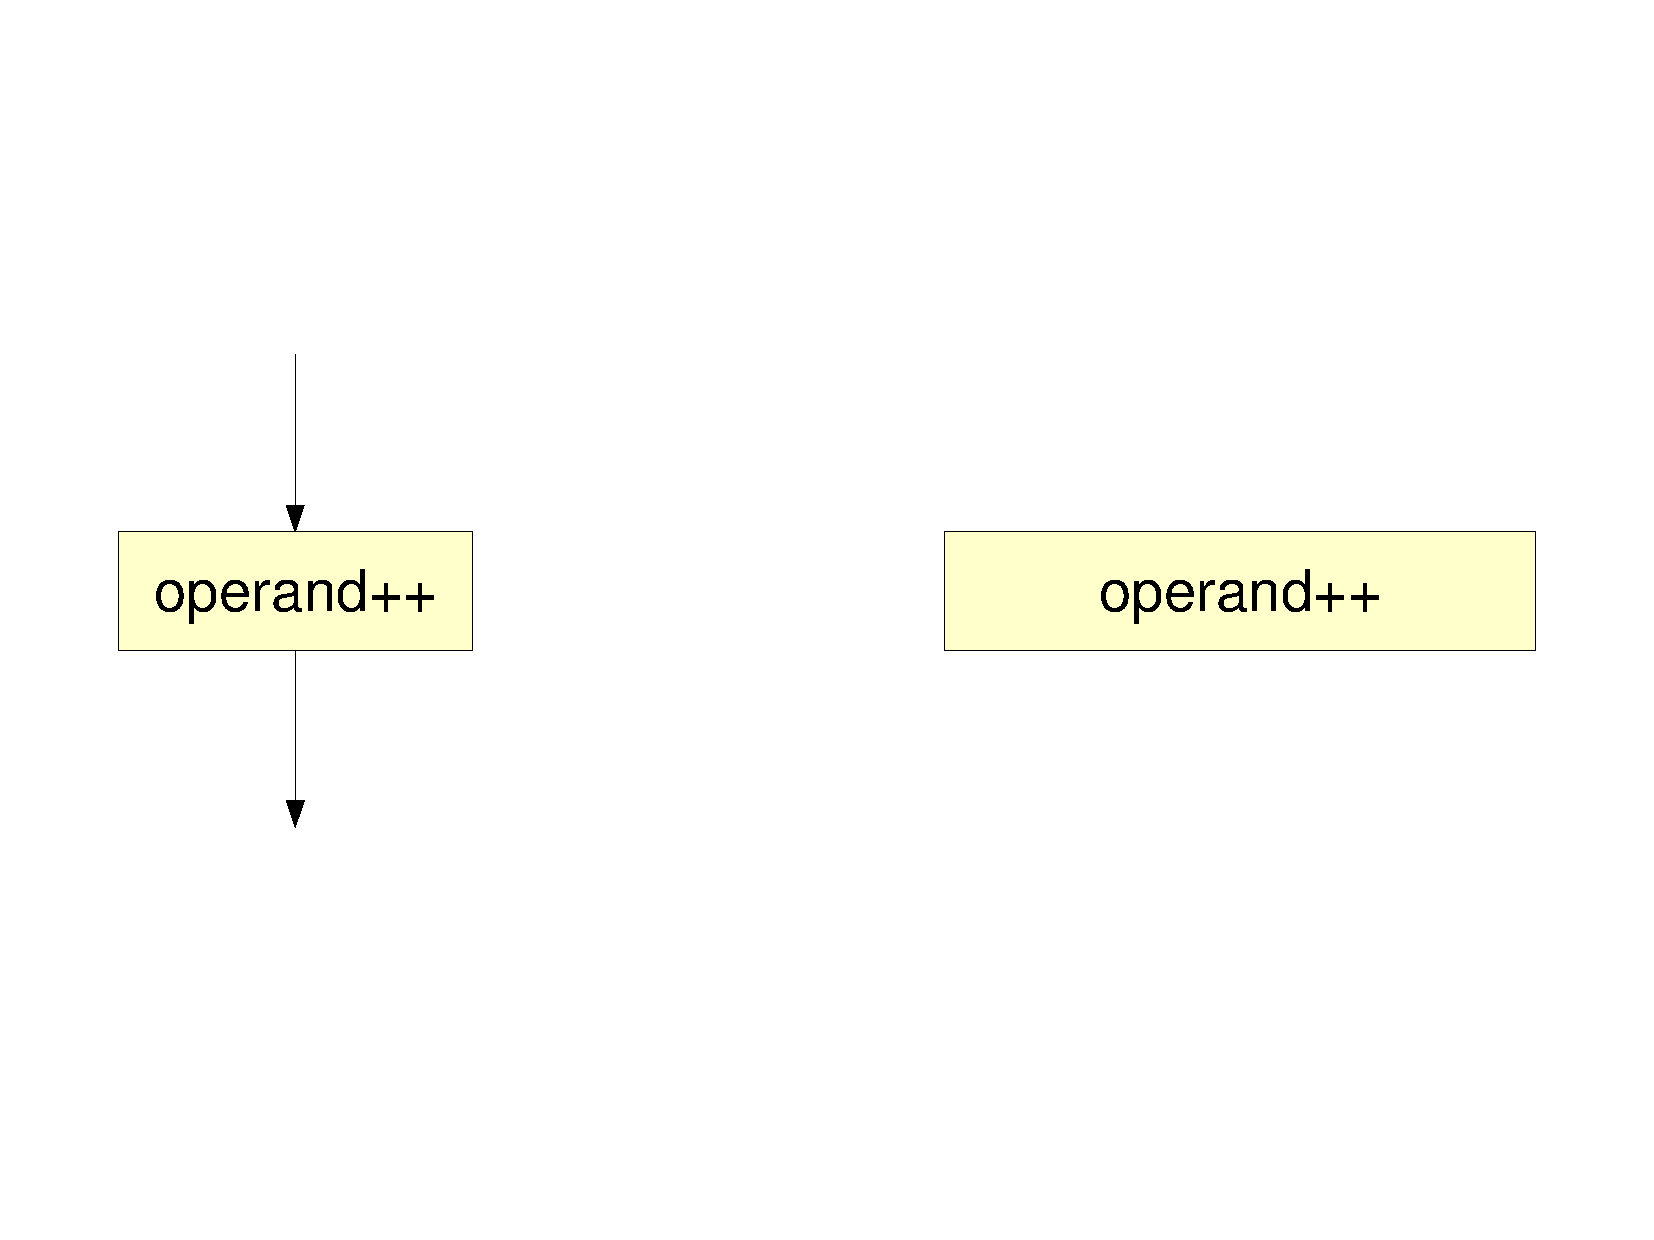
\includegraphics[scale=0.3,angle=-90]{graphic/statement.pdf}
        \caption{Statement as Program Flow Chart and Structure Chart}
        \label{statement_figure}
    \end{center}
\end{figure}

A \emph{Variable} is a placeholder for an abstracted \emph{Data Value}. It
occupies space in memory which is why this space has to be reserved before it
can be used. The reservation is called \emph{Allocation} or \emph{Declaration}
and it states the variable's \emph{Type} and an \emph{Identifier}. Commonly,
variables also get initialised through the \emph{Assignment} of an
\emph{Initial Value}. Here an example for declaration and initialisation
through assignment in \emph{C} code:

\begin{scriptsize}
    \begin{verbatim}
    type identifier = value;
    \end{verbatim}
\end{scriptsize}

Many statements which belong together can form a \emph{Block}, also called
\emph{Compound Statement}. Variables declared in a block are called its
\emph{Local Variables} and loose their validity outside that block. Blocks have
an opening and a closing symbol. Following once more an example in \emph{C}
programming language source code, showing a block with two statements:

\begin{scriptsize}
    \begin{verbatim}
    {
        statement1;
        statement2;
    }
    \end{verbatim}
\end{scriptsize}

%
% $RCSfile: branching.tex,v $
%
% Copyright (C) 2002-2008. Christian Heller.
%
% Permission is granted to copy, distribute and/or modify this document
% under the terms of the GNU Free Documentation License, Version 1.1 or
% any later version published by the Free Software Foundation; with no
% Invariant Sections, with no Front-Cover Texts and with no Back-Cover
% Texts. A copy of the license is included in the section entitled
% "GNU Free Documentation License".
%
% http://www.cybop.net
% - Cybernetics Oriented Programming -
%
% http://www.resmedicinae.org
% - Information in Medicine -
%
% Version: $Revision: 1.1 $ $Date: 2008-08-19 20:41:05 $ $Author: christian $
% Authors: Christian Heller <christian.heller@tuxtax.de>
%

\subsubsection{Branching}
\label{branching_heading}
\index{Branching}
\index{Branch}
\index{Conditional Branching}
\index{Unconditional Branching}
\index{Goto (Jump) Command}
\index{Condition}
\index{Alternative}
\index{Choice}
\index{Multiple Condition}
\index{Switch}
\index{Case}

A block of statements that get only executed at special occasions is called a
\emph{Branch}. Two kinds of branching exist: \emph{Conditional Branching} and
\emph{Unconditional Branching}. An implementation of the latter is the well-known
but also disliked \emph{goto} (\emph{jump}) command. The former depends on a
\emph{Condition}, also called \emph{Alternative} or \emph{Choice} (figure
\ref{condition_figure}), that is its statements are only executed if the
condition's result is true. That way, a condition can change the flow of a
program. A code example follows; it shows conditional branching:

\begin{scriptsize}
    \begin{verbatim}
    if (condition) {
        statements;
    } else {
        statements;
    }
    \end{verbatim}
\end{scriptsize}

\begin{figure}[ht]
    \begin{center}
        \includegraphics[scale=0.3,angle=-90]{graphic/condition.pdf}
        \caption{Condition as Program Flow Chart and Structure Chart}
        \label{condition_figure}
    \end{center}
\end{figure}

Many programming languages offer a \emph{Multiple Condition} control structure
like \emph{switch} or \emph{case}. It is a comfortable possibility to let a
program make a choice out of many alternatives:

\begin{scriptsize}
    \begin{verbatim}
    switch (condition) {
        case constant1:
            statements;
        case constant2:
            statements;
        default:
            statements;
    }
    \end{verbatim}
\end{scriptsize}

Essentially, however, it is a subsumption of a number of simple conditions which
are mostly called \emph{if-else}, and therefore replaceable by such, as shown
following:

\begin{scriptsize}
    \begin{verbatim}
    if (condition == constant1) {
        statements;
    } else if (condition == constant2) {
        statements;
    } else {
        statements;
    }
    \end{verbatim}
\end{scriptsize}

The multiple condition is conceptually no innovation in comparison with the
simple condition and hence pure convenience for the programmer. The interpreter
described in chapter \ref{cybernetics_oriented_interpreter_heading} uses solely
if-then statements.

%
% $RCSfile: looping.tex,v $
%
% Copyright (C) 2002-2008. Christian Heller.
%
% Permission is granted to copy, distribute and/or modify this document
% under the terms of the GNU Free Documentation License, Version 1.1 or
% any later version published by the Free Software Foundation; with no
% Invariant Sections, with no Front-Cover Texts and with no Back-Cover
% Texts. A copy of the license is included in the section entitled
% "GNU Free Documentation License".
%
% http://www.cybop.net
% - Cybernetics Oriented Programming -
%
% http://www.resmedicinae.org
% - Information in Medicine -
%
% Version: $Revision: 1.1 $ $Date: 2008-08-19 20:41:07 $ $Author: christian $
% Authors: Christian Heller <christian.heller@tuxtax.de>
%

\subsubsection{Looping}
\label{looping_heading}
\index{Looping}
\index{Loop Control Structure}
\index{Pre Test Loop}
\index{Post Test Loop}
\index{Counting Loop}
\index{while, while-do}
\index{do-while, repeat-until}
\index{for, for-next}

The \emph{Loop} (figure \ref{loop_figure}) is a control element that allows to
iterate through statements, in other words to execute them repeatedly, several
times. Its concept is quite simple -- a jump backwards in the program. However,
this low-level jump is hidden to the application programmer using a higher-level
SPP language. The loop is indicated by a special keyword instead, for example:

\begin{scriptsize}
    \begin{verbatim}
    while (condition) {
        statements;
    }
    \end{verbatim}
\end{scriptsize}

\begin{figure}[ht]
    \begin{center}
        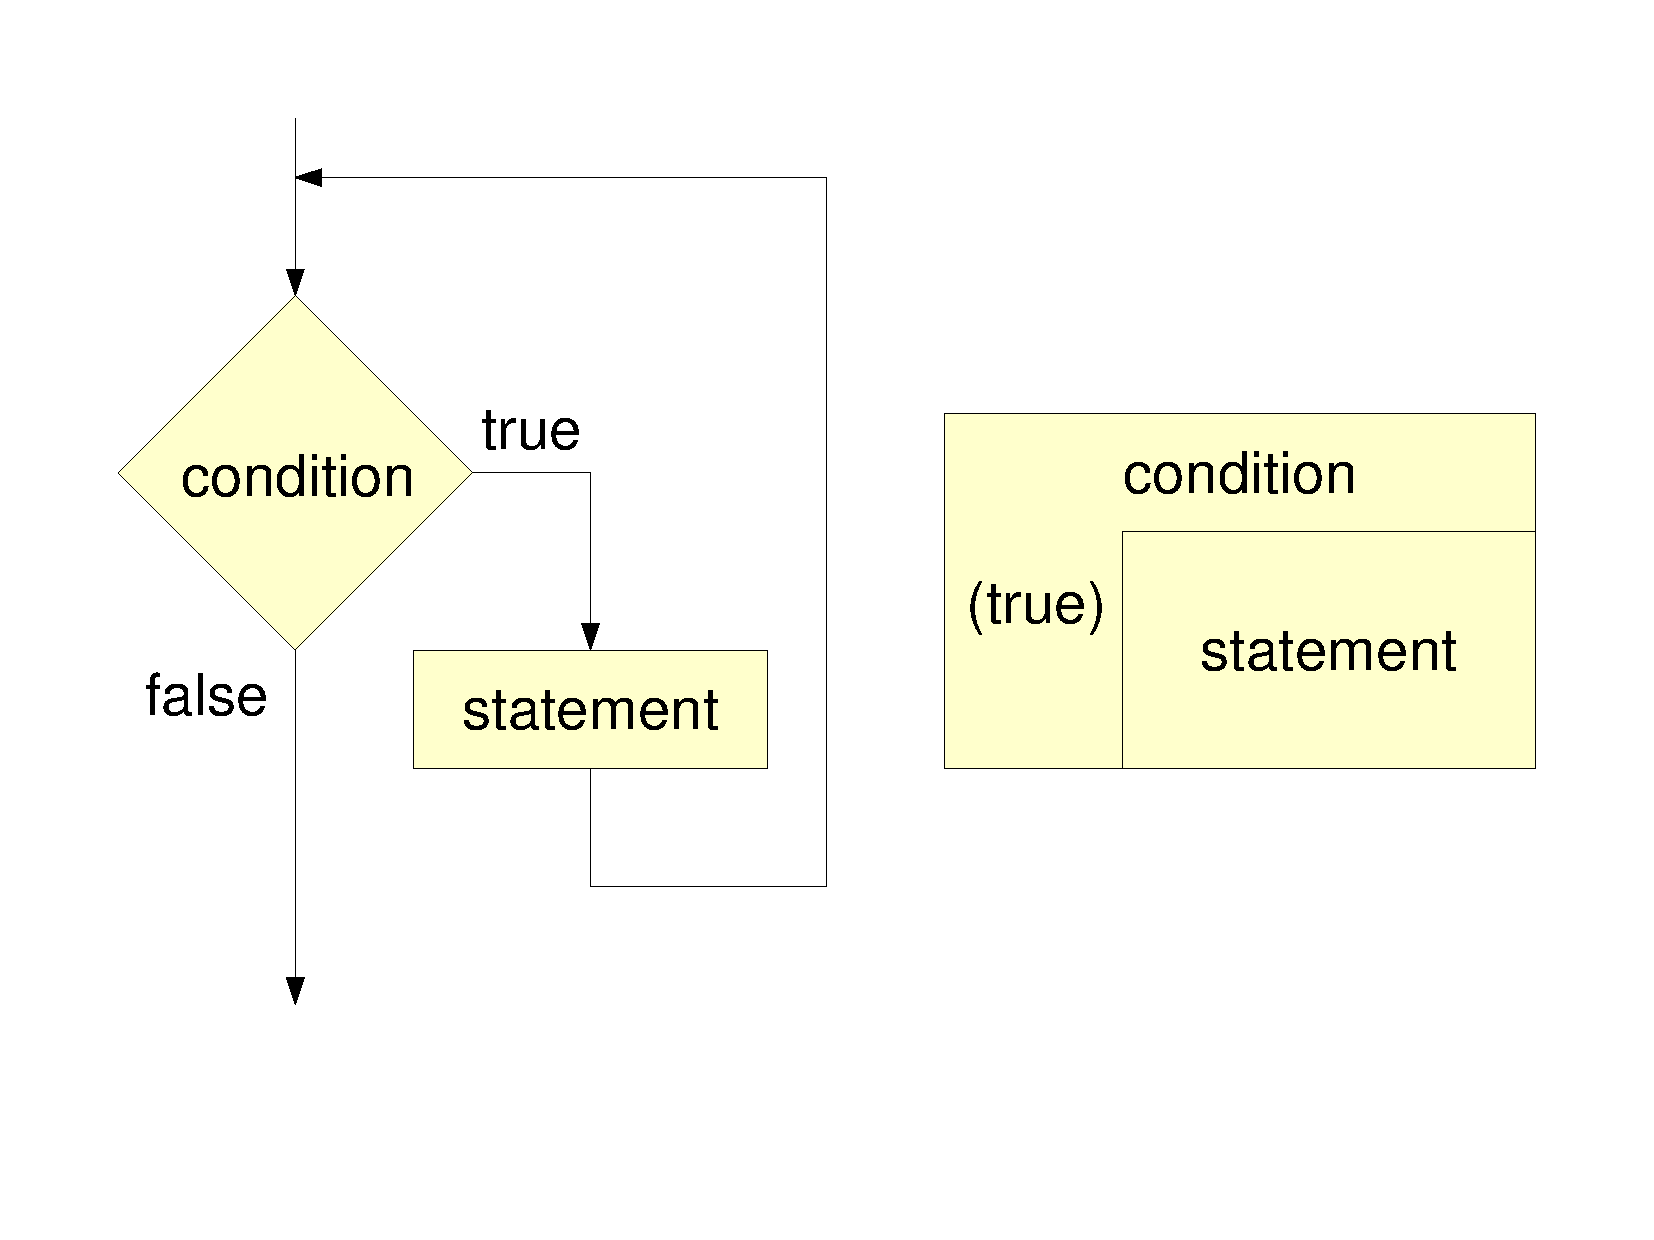
\includegraphics[scale=0.3,angle=-90]{graphic/loop.pdf}
        \caption{Loop as Program Flow Chart and Structure Chart}
        \label{loop_figure}
    \end{center}
\end{figure}

Most programming languages offer three different loop styles, as there are:

\begin{itemize}
    \item[-] Pre-test loop: \emph{while}, \emph{while-do}
    \item[-] Post-test loop: \emph{do-while}, \emph{repeat-until}
    \item[-] Counting Loop: \emph{for}, \emph{for-next}
\end{itemize}

A \emph{Pre-Test Loop} is used when one wants to check a condition before the
statements in the loop body are executed:

\begin{scriptsize}
    \begin{verbatim}
    int i = 0;
    while (i < 1) {
        statements;
        i++;
    }
    \end{verbatim}
\end{scriptsize}

The \emph{Post-Test Loop}, on the other hand, repeats all loop-body statements
until a condition is met:

\begin{scriptsize}
    \begin{verbatim}
    int i = 0;
    do {
        statements;
        i++;
    } while (i < 1);
    \end{verbatim}
\end{scriptsize}

A \emph{Counting Loop}, finally, can be applied when the number of necessary
repetitions of the loop-body statements is known in advance:

\begin{scriptsize}
    \begin{verbatim}
    int i;
    for (i = 0; i < 1; i++) {
        statements;
    }
    \end{verbatim}
\end{scriptsize}

The statements in all three loop examples are only executed once. It is not
difficult to see that the \emph{for} loop can be replaced with a \emph{while}
loop by initialising the \emph{i} variable in its declaration line and moving
the increment statement into the loop's block. But also the \emph{do-while}
loop can be replaced with a \emph{while} loop. If the behaviour does not match
(for example a while block is not executed even once), then changing the initial
loop variable value can solve this problem. Otherwise, modifying the statements
(algorithm) in the block, without changing it logically, will do.

As can be seen: Most variations of the \emph{Looping} concept are just a
convenience for the programmer. They are conceptually identical and can be lead
back to a simple loop with break condition, each. The interpreter described in
chapter \ref{cybernetics_oriented_interpreter_heading} uses just one kind of
loop.


%
% $RCSfile: system_programming.tex,v $
%
% Copyright (C) 2002-2008. Christian Heller.
%
% Permission is granted to copy, distribute and/or modify this document
% under the terms of the GNU Free Documentation License, Version 1.1 or
% any later version published by the Free Software Foundation; with no
% Invariant Sections, with no Front-Cover Texts and with no Back-Cover
% Texts. A copy of the license is included in the section entitled
% "GNU Free Documentation License".
%
% http://www.cybop.net
% - Cybernetics Oriented Programming -
%
% http://www.resmedicinae.org
% - Information in Medicine -
%
% Version: $Revision: 1.1 $ $Date: 2008-08-19 20:41:09 $ $Author: christian $
% Authors: Christian Heller <christian.heller@tuxtax.de>
%

\subsection{System Programming}
\label{system_programming_heading}
\index{System Programming}
\index{System Programming Language}
\index{PL/1}
\index{Pascal}
\index{C}
\index{C++}
\index{Java}
\index{LISP}
\index{Fortran}
\index{Algol}
\index{Assembly Language}
\index{Strong Typing}
\index{Static Typing}
\index{Typing}

After John K. Ousterhout \cite{ousterhout1998}, \emph{System Programming Languages}
such as \emph{PL/1}, \emph{Pascal}, \emph{C} or \emph{C++} or \emph{Java}
(which evolved from higher level languages such as \emph{LISP}, \emph{Fortran} or
\emph{Algol} -- see section \ref{language_history_heading}) had been introduced
as an alternative to \emph{Assembly Languages} and both would differ in two
ways. While in an assembly language, virtually every aspect of a machine were
reflected in the program, each statement representing a single machine
instruction so that programmers had to deal with low-level details such as
register allocation and procedure calling sequences, a system programming
language were:

\begin{enumerate}
    \item \emph{higher level} because its statements did not correspond exactly
        to machine instructions; a compiler would translate each statement in
        the source program into a sequence of binary instructions and handle
        register allocation;
    \item \emph{strongly typed} because programmers needed to declare how each
        piece of information would be used; the language would prevent the
        information from being used in any other way.
\end{enumerate}

Ousterhout uses the term \emph{Typing} to: \textit{refer to the degree to which
the meaning of information is specified in advance of its use}. After him, the
strong typing (also called \emph{Static Typing}) of today's system programming
languages had several advantages, such as:

\begin{itemize}
    \item[-] Better manageability of large programs by differentiating between
        things that must be treated differently
    \item[-] Possible error detection by using type information in compilers
    \item[-] Improved performance by allowing compilers to generate specialized code
\end{itemize}

But there were also a number of disadvantages when using system programming
languages:

\begin{itemize}
    \item[-] Need to declare each variable with a particular type and to use it
        in ways that are appropriate for the type
    \item[-] Difficulty to create new code on the fly due to total segregation
        of data and code
    \item[-] Impossibility to use an object of one type where an object of a
        different type is expected, because variables are collected in objects
        with well-defined substructure and procedures to manipulate them
\end{itemize}

%
% $RCSfile: typeless_programming.tex,v $
%
% Copyright (C) 2002-2008. Christian Heller.
%
% Permission is granted to copy, distribute and/or modify this document
% under the terms of the GNU Free Documentation License, Version 1.1 or
% any later version published by the Free Software Foundation; with no
% Invariant Sections, with no Front-Cover Texts and with no Back-Cover
% Texts. A copy of the license is included in the section entitled
% "GNU Free Documentation License".
%
% http://www.cybop.net
% - Cybernetics Oriented Programming -
%
% http://www.resmedicinae.org
% - Information in Medicine -
%
% Version: $Revision: 1.1 $ $Date: 2008-08-19 20:41:09 $ $Author: christian $
% Authors: Christian Heller <christian.heller@tuxtax.de>
%

\subsection{Typeless Programming}
\label{typeless_programming_heading}
\index{Typeless Programming}
\index{Scripting Language}
\index{Job Control Language}
\index{Batch Language}
\index{Perl}
\index{Python}
\index{Rexx}
\index{Tcl}
\index{Visual Basic}
\index{VB}
\index{Universal Interactive Executive}
\index{UNIX}
\index{Script Oriented Programming}
\index{SOP}
\index{Dynamic Typing}
\index{System Integration Language}
\index{Glue Language}

\emph{Scripting Languages} (formerly also called \emph{Job Control-} or
\emph{Batch Languages} \cite{wikipedia}) such as Perl \cite{wall}, Python
\cite{lutz}, Rexx \cite{ohara}, Tcl \cite{ousterhout1994}, \emph{Visual Basic}
(VB) and the \emph{Universal Interactive Executive} (UNIX) shells overcome the
disadvantages of system programming languages (section
\ref{system_programming_heading}) by being \emph{typeless} and
\emph{interpreted}. The paradigm behind them is sometimes called
\emph{Script Oriented Programming} (SOP).

Ousterhout \cite{ousterhout1998} writes that modern computers were fundamentally
typeless: any word in memory could hold any kind of value, such as an integer, a
floating-point number, a pointer, or an instruction. The meaning of a value were
determined by how it is used: if the program counter pointed at a word of memory
then it were treated as an instruction; if a word were referenced by an integer
\emph{add} instruction then it were treated as an integer; and so on. The same
word could be used in different ways at different times (what is also called
\emph{Dynamic Typing}).

Because scripting languages are intended primarily for plugging together existing
components, they are also referred to as \emph{System Integration Languages} or
\emph{Glue Languages}. They provide a higher level of programming than assembly-
or system programming languages. Through their usage, integrated applications,
after \cite{ousterhout1998}, could be developed five to ten times faster than
with system programming languages. Scripting languages sacrifice execution speed
to improve development speed.

The interpreter described in chapter \ref{cybernetics_oriented_interpreter_heading}
is able to handle data (knowledge) without knowing about their type (kind of
abstraction) in advance, that is at compilation time. Although itself written
in the system programming language \emph{C}, the interpreter is very flexible
when it comes to processing knowledge.

%
% $RCSfile: functional_programming.tex,v $
%
% Copyright (C) 2002-2008. Christian Heller.
%
% Permission is granted to copy, distribute and/or modify this document
% under the terms of the GNU Free Documentation License, Version 1.1 or
% any later version published by the Free Software Foundation; with no
% Invariant Sections, with no Front-Cover Texts and with no Back-Cover
% Texts. A copy of the license is included in the section entitled
% "GNU Free Documentation License".
%
% http://www.cybop.net
% - Cybernetics Oriented Programming -
%
% http://www.resmedicinae.org
% - Information in Medicine -
%
% Version: $Revision: 1.1 $ $Date: 2008-08-19 20:41:06 $ $Author: christian $
% Authors: Christian Heller <christian.heller@tuxtax.de>
%

\subsection{Functional Programming}
\label{functional_programming_heading}
\index{Functional Programming}
\index{Lisp}
\index{Automatic Storage Management}
\index{Integrated Development Environment}
\index{Prolog}
\index{Pascal}
\index{C}
\index{Special Purpose Language}
\index{SPL}
\index{General Purpose Language}
\index{GPL}
\index{Imperative Language}
\index{Functional Language}
\index{Haskell}
\index{Side Effect}
\index{SML}
\index{Scheme}
\index{Association of Lisp Users}

Many languages such as \emph{Lisp} and its relatives cannot be characterised
cleanly as system programming language or scripting language; they are situated
somewhere between. Concepts like \emph{Interpretation} and \emph{Dynamic Typing},
now common in scripting languages, stem from Lisp \cite{ousterhout1998}. Others like
\emph{Automatic Storage Management} and \emph{Integrated Development Environments},
now used in both scripting- and system programming languages, were introduced by
Lisp as well. Peter Norvig writes in \cite{norvig}:

\begin{quote}
    There is a myth that Lisp (and Prolog) are \emph{Special Purpose Languages}
    (SPL), while languages such as Pascal and C are \emph{General Purpose} (GPL).
    Actually, just the reverse is true. Pascal and C are special-purpose languages
    for manipulating the registers and memory of a \emph{von Neumann}-style computer.
    The majority of their syntax is devoted to arithmetic and Boolean expressions,
    and while they provide some facilities for forming data structures, they have
    poor mechanisms for procedural abstraction or control abstraction. In addition,
    they are designed for the \emph{state-oriented} style of programming: computing
    a result by changing the value of variables through assignment statements.
\end{quote}

The \emph{Frequently Asked Questions} (FAQ) edited by Graham Hutton \cite{hutton}
distinguish between \emph{Imperative Languages} and \emph{Functional Languages}.
System programming languages as introduced in previous sections belong to the
first group. To calculate the sum of the integers from 1 to 10, for example,
they would probably use a simple loop and repeatedly update the values held in
an accumulator variable \emph{total} and a counter variable \emph{i}:

\begin{scriptsize}
    \begin{verbatim}
    int total = 0;
    for (int i = 1; i <= 10; ++i) {
        total += i;
    }
    \end{verbatim}
\end{scriptsize}

A functional language like \emph{Haskell} would express the same program
\emph{without} any variable updates, by evaluating an expression, as shown
below. Variable updates, that is \textit{computational effects caused by
expression evaluation that persist after the evaluation is completed}
\cite{hutton} are called \emph{Side Effects}.

\begin{scriptsize}
    \begin{verbatim}
    sum [1..10]
    \end{verbatim}
\end{scriptsize}

The following two examples \cite{hutton} show the same program in two other
functional languages, namely \emph{SML} and \emph{Scheme}:

\begin{scriptsize}
    \begin{verbatim}
    let fun sum i tot = if i = 0 then tot else sum (i - 1) (tot + i)
    in sum 10 0
    end
    \end{verbatim}
\end{scriptsize}

\begin{scriptsize}
    \begin{verbatim}
    (define sum
    (lambda (from total)
        (if (= 0 from)
            total
            (sum (- from 1) (+ total from)))))
    (sum 10 0)
    \end{verbatim}
\end{scriptsize}

The \emph{Association of Lisp Users} \cite{commonlisp} points out the absence
of side effects and explains \emph{Functional Programming} as follows:

\begin{quote}
    Functional programming describes all computer operations as mathematical
    functions on inputs. Typically, a function can be created and returned from
    other functions as first-class data. This function object may then be passed
    as input to other functions, perhaps be composed with other functions, and
    eventually, applied to inputs to produce a value. Objects can be defined in
    terms of functions that encapsulate certain data, and operations on objects
    can be defined by functions encapsulating the objects. Purely functional
    languages do not have assignment, as all side-effecting can be defined in
    terms of functions that encapsulate the changed data. Procedural languages
    essentially perform everything as side-effects to data structures. A purely
    procedural language would have no functions, but might have subroutines of
    no arguments that returned no values, and performed certain assignments and
    other operations based on the data it found stored in the system.
\end{quote}

The interpreter described in chapter \ref{cybernetics_oriented_interpreter_heading}
manipulates \emph{all} data (knowledge) as if it would be one huge side effect.
Data (knowledge models) are not bundled with-, but kept completely outside any
functions/ procedures. Only references to these data are handed over as
parameters.

%
% $RCSfile: logical_programming.tex,v $
%
% Copyright (C) 2002-2008. Christian Heller.
%
% Permission is granted to copy, distribute and/or modify this document
% under the terms of the GNU Free Documentation License, Version 1.1 or
% any later version published by the Free Software Foundation; with no
% Invariant Sections, with no Front-Cover Texts and with no Back-Cover
% Texts. A copy of the license is included in the section entitled
% "GNU Free Documentation License".
%
% http://www.cybop.net
% - Cybernetics Oriented Programming -
%
% http://www.resmedicinae.org
% - Information in Medicine -
%
% Version: $Revision: 1.1 $ $Date: 2008-08-19 20:41:07 $ $Author: christian $
% Authors: Christian Heller <christian.heller@tuxtax.de>
%

\subsection{Logical Programming}
\label{logical_programming_heading}
\index{Logical Programming}
\index{Declarative Programming}
\index{Artificial Intelligence}
\index{AI}
\index{Expert System}
\index{Automated Theorem Proving}
\index{Monkey and Banana Problem}
\index{Prolog}
\index{Mercury}
\index{TyRuBa}

\emph{Functional Programming} as introduced in the previous section is one kind
of \emph{Declarative Programming}, which describes to the computer a set of
conditions and lets the computer figure out how to satisfy them \cite{wikipedia}.
Another kind is \emph{Logical Programming}. It specifies a set of attributes
that a solution should have -- rather than a set of steps to obtain such a
solution. Schematically, the logical programming process follows the equation:

\begin{scriptsize}
    \begin{verbatim}
    facts + rules = results
    \end{verbatim}
\end{scriptsize}

Logical programming was strongly influenced by \emph{Artificial Intelligence}
(AI) and is applied in domains such as \emph{Expert Systems}, where the program
generates a recommendation or answer from a large model of the application
domain, and \emph{Automated Theorem Proving}, where the program generates novel
theorems to extend some existing body of theory. \cite{wikipedia}

The \emph{Monkey and Banana Problem} is a famous example studied in the community
of logical programming \cite{wikipedia}: \textit{Instead of the programmer
explicitly specifying the path for the monkey to reach the banana, the computer
actually reasons out a possible way that the monkey reaches the banana.}

A prominent logical language representative is \emph{Prolog}; a more recent one
is \emph{Mercury}; an \emph{Open Source Software} (OSS) one is \emph{TyRuBa}.

%
% $RCSfile: data_manipulation_language.tex,v $
%
% Copyright (C) 2002-2008. Christian Heller.
%
% Permission is granted to copy, distribute and/or modify this document
% under the terms of the GNU Free Documentation License, Version 1.1 or
% any later version published by the Free Software Foundation; with no
% Invariant Sections, with no Front-Cover Texts and with no Back-Cover
% Texts. A copy of the license is included in the section entitled
% "GNU Free Documentation License".
%
% http://www.cybop.net
% - Cybernetics Oriented Programming -
%
% http://www.resmedicinae.org
% - Information in Medicine -
%
% Version: $Revision: 1.1 $ $Date: 2008-08-19 20:41:06 $ $Author: christian $
% Authors: Christian Heller <christian.heller@tuxtax.de>
%

\subsection{Data Manipulation Language}
\label{data_manipulation_language_heading}
\index{Data Manipulation Language}
\index{DML}
\index{Structured Query Language}
\index{SQL}
\index{Structured English Query Language}
\index{SEQUEL}
\index{Relational Database Management System}
\index{RDBMS}
\index{Data Definition Language}
\index{DDL}
\index{Data Control Language}
\index{DCL}

A \emph{Data Manipulation Language} (DML), after \cite{wikipedia}, is:
\textit{a family of computer languages used by computer programs or database
users to retrieve, insert, delete and update data in a database}. As most
popular DML, the source mentions the \emph{Structured Query Language} (SQL)
that was originally developed as \emph{Structured English Query Language}
(SEQUEL) by \emph{International Business Machines} (IBM), after the model
described by Edgar F. Codd in \cite{codd}.

Technically, SQL is a set-based, declarative computer language that, after
\cite{wikipedia}, could be used to create, modify and retrieve data from
\emph{Relational Database Management Systems} (RDBMS). Its keywords are often
shared into the three groups:

\begin{itemize}
    \item[-] \emph{Data Manipulation Language} (DML): SELECT, INSERT, UPDATE, DELETE
    \item[-] \emph{Data Definition Language} (DDL): CREATE, DROP
    \item[-] \emph{Data Control Language} (DCL): GRANT, REVOKE
\end{itemize}

Since the details of that language are outside the scope of this work, they are
not elaborated further here, but can be learned at for example \cite{sqltutorial}.
%The \emph{Entity Relationship Model} (ERM) as basic data model behind
%\emph{Relational Database Management Systems} (RDBMS) (section
%\ref{database_server_heading}), however, is described briefly in section
%\ref{entity_relationship_model_heading}.

%
% $RCSfile: markup_language.tex,v $
%
% Copyright (C) 2002-2008. Christian Heller.
%
% Permission is granted to copy, distribute and/or modify this document
% under the terms of the GNU Free Documentation License, Version 1.1 or
% any later version published by the Free Software Foundation; with no
% Invariant Sections, with no Front-Cover Texts and with no Back-Cover
% Texts. A copy of the license is included in the section entitled
% "GNU Free Documentation License".
%
% http://www.cybop.net
% - Cybernetics Oriented Programming -
%
% http://www.resmedicinae.org
% - Information in Medicine -
%
% Version: $Revision: 1.1 $ $Date: 2008-08-19 20:41:07 $ $Author: christian $
% Authors: Christian Heller <christian.heller@tuxtax.de>
%

\subsection{Markup Language}
\label{markup_language_heading}
\index{Markup Language}
\index{World Wide Web}
\index{WWW}
\index{Style of a Document}
\index{Structure of a Document}
\index{Content of a Document}
\index{TeX}
\index{Lamport TeX}
\index{LaTeX}
\index{LaTeXe}
\index{Scribe}
\index{Standard Generalized Markup Language}
\index{SGML}
\index{Extensible Markup Language}
\index{XML}
\index{Hypertext Markup Language}
\index{HTML}
\index{DocBook}
\index{Text Encoding Initiative}
\index{TEI}

At latest with the distribution of the \emph{World Wide Web} (WWW),
\emph{Markup Languages} increasingly gained in popularity. A markup language
separates the presentation \emph{Style} of a document from its logical
\emph{Structure} and \emph{Content}. Well-known representatives of markup
languages, two famous of which being described in the following sections, are
\cite{wikipedia}:

\begin{itemize}
    \item[-] \emph{\TeX} / \emph{Lamport \TeX} (\LaTeX, \LaTeXe)
    \item[-] \emph{Scribe}
    \item[-] \emph{Standard Generalized Markup Language} (SGML)
    \item[-] \emph{Extensible Markup Language} (XML)
    \item[-] \emph{Hypertext Markup Language} (HTML)
    \item[-] \emph{DocBook}
    \item[-] \emph{Text Encoding Initiative} (TEI)
\end{itemize}

Recently, more and more projects appear that try to use markup languages not
just for document markup, but also for declarative programming.% More on this in
%section \ref{xml_based_programming_heading}.
Before coming to the actual markup languages, the paradigm of
\emph{Literate Programming} and its idea to use markup tokens for distinguishing
source code and documentation, is investigated.

%
% $RCSfile: literate_programming.tex,v $
%
% Copyright (C) 2002-2008. Christian Heller.
%
% Permission is granted to copy, distribute and/or modify this document
% under the terms of the GNU Free Documentation License, Version 1.1 or
% any later version published by the Free Software Foundation; with no
% Invariant Sections, with no Front-Cover Texts and with no Back-Cover
% Texts. A copy of the license is included in the section entitled
% "GNU Free Documentation License".
%
% http://www.cybop.net
% - Cybernetics Oriented Programming -
%
% http://www.resmedicinae.org
% - Information in Medicine -
%
% Version: $Revision: 1.1 $ $Date: 2008-08-19 20:41:07 $ $Author: christian $
% Authors: Christian Heller <christian.heller@tuxtax.de>
%

\subsubsection{Literate Programming}
\label{literate_programming_heading}
\index{Literate Programming}
\index{Token Character}
\index{Commercial At @}
\index{Re-ordering of Code}
\index{Typeset Code and Documentation}
\index{Cross Referencing}
\index{Source Code Documentation}
\index{JavaDoc}
\index{Doxygen}
\index{DOC++}

Ross Williams writes in \cite[section 1.1]{williams}:

\begin{quote}
    A traditional computer program consists of a text file containing program
    code. Scattered in amongst the program code are comments which describe the
    various parts of the code. In \emph{Literate Programming}, the emphasis is
    reversed. Instead of writing code containing documentation, the literate
    programmer writes documentation containing code.
\end{quote}

In other words, \emph{Literate Programming} pays more attention to proper source
code documentation than classical programming languages do. It mostly offers
special \emph{Token} characters like the \emph{Commercial At} character \emph{@}
for example, which serve as code delimiters. The delimited blocks are determined
by particular tools such as a preprocessor that filters out program code to be
processed further. All source information together (input document, commentaries,
program code) is used to generate typeset documentation files in one or more
formats.

Williams \cite{williams} means that the literate programming system provided
far more than: \textit{just a reversal of the priority of comments and code.}
In its full-blown form, a good literate programming facility could provide:

\begin{itemize}
    \item[-] \emph{Re-ordering of Code:} Some programming languages force the
        programmer to give the various program parts in a particular order.
    \item[-] \emph{Typeset Code and Documentation:} Because a literate programming
        utility sees all the code, it can use its knowledge of the programming
        language and the features of the typesetting language to typeset the
        program code as if it were appearing in a technical journal.
    \item[-] \emph{Cross referencing:} Because a literate tool sees all the code
        and documentation, it is able to generate extensive cross referencing
        information in the typeset documentation, which makes the printed program
        document more easy to navigate and partially compensates for the lack of
        an automatic searching facility when reading printed documentation.
\end{itemize}

It is true, the actual instructions and algorithms in between commentaries are
written in (or translated into) a system programming- or other kind of language.
But literate programming places its focus on source code \emph{Documentation}
for which it uses \emph{Markup} tokens, which is why it was classified under
\emph{Markup Language} in this work.

Although literate programming itself has not gained that much popularity, its
idea of using markup tokens to generate more expressive source code documentation
has. Several up-to-date programming environments make use of it. A well-known
example is the \emph{JavaDoc} tool \cite{javadoc}; other systems are
\emph{Doxygen} \cite{doxygen} or \emph{DOC++} \cite{docpp}.

%
% $RCSfile: tex_and_latex.tex,v $
%
% Copyright (C) 2002-2008. Christian Heller.
%
% Permission is granted to copy, distribute and/or modify this document
% under the terms of the GNU Free Documentation License, Version 1.1 or
% any later version published by the Free Software Foundation; with no
% Invariant Sections, with no Front-Cover Texts and with no Back-Cover
% Texts. A copy of the license is included in the section entitled
% "GNU Free Documentation License".
%
% http://www.cybop.net
% - Cybernetics Oriented Programming -
%
% http://www.resmedicinae.org
% - Information in Medicine -
%
% Version: $Revision: 1.1 $ $Date: 2008-08-19 20:41:09 $ $Author: christian $
% Authors: Christian Heller <christian.heller@tuxtax.de>
%

\subsubsection{TeX and LaTeX}
\label{tex_and_latex_heading}
\index{Tex}
\index{Lamport TeX}
\index{LaTeX}
\index{LaTeXe}
\index{Device Independent Format}
\index{DVI}
\index{PDFTeX}
\index{Portable Document Format}
\index{PDF}
\index{TeX User Group}
\index{TUG}
\index{Desktop Publishing}
\index{DTP}

The special-purpose \TeX\ \cite{tex} language is the centre-piece of a
typesetting system which, due to its well-formatted output of complex
mathematical formulas and generally high-quality typesetting, is especially
popular among academic circles of mathematicians, physicists and computer
scientists \cite{latextutorial}. The Wikipedia encyclopedia \cite{wikipedia}
writes:

\begin{quote}
    \TeX\ is a macro and token based language: many commands, including most
    user-defined ones, are expanded on the fly until only unexpandable tokens
    remain which get executed. Expansion itself is practically side-effect free.
    Tail recursion of macros takes no memory, and if-then-else constructs are
    available. \ldots

    The \TeX\ system has precise knowledge of the sizes of all characters and
    symbols, and using this information, it computes the optimal arrangement of
    letters per line and lines per page. It then produces a \emph{Device Independent}
    (DVI) file containing the final locations of all characters. The DVI file
    can be printed directly given an appropriate printer driver, or it can be
    converted to other formats.
\end{quote}

The \emph{PDFTeX} translator program is often used to bypass all DVI generation,
by creating \emph{Portable Document Format} (PDF) files directly.

Nowadays, \TeX\ is mostly used with a template extension called \emph{Lamport \TeX}
(\LaTeX, \LaTeXe) \cite{latex}. The Indian \emph{\TeX\ Users Group} (TUG) writes
\cite{latextutorial}: \textit{\LaTeX\ is a document preparation system which
adds a set of functions that make the \TeX\ language friendlier than using
the primitives provided by it.} It offers programmable \emph{Desktop Publishing}
(DTP) features and extensive facilities for automating most aspects of
typesetting. \cite{wikipedia}

The most important feature of \TeX\ for this work is its kind of relating meta-
with structural information. Two examples may help here:

\begin{scriptsize}
    \begin{verbatim}
    \documentclass[a4paper,12pt]{book}
    \includegraphics[scale=0.3]{path/file.pdf}
    \end{verbatim}
\end{scriptsize}

The first statement determines \emph{book} as document class for a document to
be written. It contains additional information such as paper- and font size, in
square brackets. The second statement refers to a graphics file to be included.
The additional information given in square brackets here is the scale factor.
With a different syntax, but in a comparable manner, the knowledge modelling
language introduced in chapter \ref{cybernetics_oriented_language_heading} does
relate structural- with meta information.

%
% $RCSfile: extensible_markup_language.tex,v $
%
% Copyright (C) 2002-2008. Christian Heller.
%
% Permission is granted to copy, distribute and/or modify this document
% under the terms of the GNU Free Documentation License, Version 1.1 or
% any later version published by the Free Software Foundation; with no
% Invariant Sections, with no Front-Cover Texts and with no Back-Cover
% Texts. A copy of the license is included in the section entitled
% "GNU Free Documentation License".
%
% http://www.cybop.net
% - Cybernetics Oriented Programming -
%
% http://www.resmedicinae.org
% - Information in Medicine -
%
% Version: $Revision: 1.1 $ $Date: 2008-08-19 20:41:06 $ $Author: christian $
% Authors: Christian Heller <christian.heller@tuxtax.de>
%

\subsubsection{Extensible Markup Language}
\label{extensible_markup_language_heading}
\index{Extensible Markup Language}
\index{XML}
\index{World Wide Web}
\index{WWW}
\index{World Wide Web Consortium}
\index{W3C}
\index{Standard Generalized Markup Language}
\index{SGML}
\index{Hypertext Markup Language}
\index{HTML}
\index{Document Publishing}
\index{Data Transfer}
\index{GUI Design}
\index{Workflow Composition}
\index{Database Storage}
\index{Domain Modelling}

A popular, very flexible, yet simple language playing an increasingly important
role in the exchange of a wide variety of data on the \emph{World Wide Web}
(WWW) and elsewhere is the \emph{Extensible Markup Language} (XML) \cite{xml},
defined by the \emph{World Wide Web Consortium} (W3C) \cite{w3c}. Being a text
format derived as simplified subset (dialect) of the
\emph{Standard Generalized Markup Language} (SGML) \cite{sgml}, it allows to
structure and store information hierarchically as \emph{Document} file. Norman
Walsh \cite{walsh} writes:

\begin{quote}
    A markup language is a mechanism to \emph{identify structures} in a document.
    The XML specification defines a standard way to \emph{add markup} to documents.
\end{quote}

And the XML Cover Pages \cite{sgmlmetamarkup} state:

\begin{quote}
    Both SGML and XML are \emph{meta} languages because they are used for
    defining \emph{markup} languages. A markup language defined using SGML or
    XML has a specific vocabulary (labels for elements and attributes) and a
    declared syntax (grammar defining the hierarchy and other features).
\end{quote}

Historically, markup languages became widely known through the
\emph{Hypertext Markup Language} (HTML) as language of the Web. To overcome its
limitations, XML was originally \emph{designed to meet the challenges of large-
scale electronic publishing} \cite{xml}. Today, XML is applied in many different
areas, for example:

\begin{itemize}
    \item[-] Document Publishing \cite{docbook}
    \item[-] Data Transfer \cite{soap}
    \item[-] GUI Design \cite{xul, uiml, ecml, xaml}
    \item[-] Workflow Composition \cite{oio, intershop}
    \item[-] Database Storage \cite{exist, dbxml}
    \item[-] Domain Modelling \cite{xmlschema, damloil}
\end{itemize}

Yet in the opinion of Robin Cover \cite{xmlsemantics}, the usability of XML for
domain modelling is limited. He writes:

\begin{quote}
    Just like its parent metalanguage (SGML), XML has no formal mechanism to
    support the declaration of semantic integrity constraints, and XML processors
    have no means of validating object semantics even if these are declared
    informally in an XML DTD. XML processors will have no inherent understanding
    of document object semantics because XML (meta-)markup languages have no
    predefined application-level processing semantics. XML thus formally governs
    syntax only -- not semantics.

    In fact, XML syntax is designed for representing an encoded serialization,
    and thus has a very limited range of expression for modeling complex object
    semantics, where \emph{Semantics} fundamentally means an intricate web of
    constrained relationships and properties. Otherwise stated: XML is a poor
    language for data modelling \ldots
\end{quote}

The XML-based language described in chapter \ref{cybernetics_oriented_language_heading}
proves the opposite. By applying a common knowledge modelling schema (chapter
\ref{knowledge_schema_heading}), it allows to model arbitrary meta information
(complex object semantics). Robin Cover continues \cite{xmlsemantics}:

\begin{quote}
    The notion of \emph{Attribute} might have been more useful except that XML
    supports only a flat data model for the value of an attribute in a
    name-value pair (essentially \emph{String}). This flat model cannot easily
    capture complex attribute notions such as would be predicated of abstracted
    real world objects, where attribute values are themselves typically
    represented by complex objects, either owned or referenced.
\end{quote}

This criticism of Cover is absolutely correct. It can be circumvented, though.
The language introduced in chapter \ref{cybernetics_oriented_language_heading}
permits one attribute to store a (file) path to an external compound knowledge
template and is thus capable of representing compound properties (complex
attribute notions). One problem remains, however: When serialising compound
knowledge models consisting of other compound models, the quotation mark as
attribute value delimiter is not sufficient, because the beginning and end of
an attribute value may get mixed up. Solving it, the XML standard needs to be
injured (chapter \ref{cybernetics_oriented_language_heading}).


%
% $RCSfile: page_description_language.tex,v $
%
% Copyright (C) 2002-2008. Christian Heller.
%
% Permission is granted to copy, distribute and/or modify this document
% under the terms of the GNU Free Documentation License, Version 1.1 or
% any later version published by the Free Software Foundation; with no
% Invariant Sections, with no Front-Cover Texts and with no Back-Cover
% Texts. A copy of the license is included in the section entitled
% "GNU Free Documentation License".
%
% http://www.cybop.net
% - Cybernetics Oriented Programming -
%
% http://www.resmedicinae.org
% - Information in Medicine -
%
% Version: $Revision: 1.1 $ $Date: 2008-08-19 20:41:08 $ $Author: christian $
% Authors: Christian Heller <christian.heller@tuxtax.de>
%

\subsection{Page Description Language}
\label{page_description_language_heading}
\index{Page Description Language}
\index{PDL}
\index{Device Independent Format}
\index{DVI}
\index{Printer Control Language}
\index{PCL}
\index{PostScript}
\index{PS}
\index{Portable Document Format}
\index{PDF}

In order to be (more or less) complete in the language overview given in this
work, the \emph{Page Description Language} (PDL) as further category shall be
mentioned here as well. It describes the contents and appearance (text,
graphical shapes, images) of a page to be printed in a device-independent,
higher-level way than an actual output bitmap \cite{wikipedia}. It may
therefore serve as an: \textit{interchange standard for (the) transmission and
storage of printable documents} \cite{foldoc}. Well-known PDL representatives
are:

\begin{itemize}
    \item[-] \emph{Device Independent} (DVI) format
    \item[-] \emph{Printer Control Language} (PCL)
    \item[-] \emph{PostScript} (PS)
    \item[-] \emph{Portable Document Format} (PDF)
\end{itemize}

After \cite{foldoc}, \emph{PostScript} is a: \textit{full programming language,
rather than a series of low-level escape sequences}. It is stack-based and
interpreted. These properties made it the: \textit{language of choice for
graphical output, until PDF appeared}. The following PostScript code example
\cite{wikipedia} computes (3 + 4) * (5 - 1):

\begin{scriptsize}
    \begin{verbatim}
    3 4 add 5 1 sub mul
    \end{verbatim}
\end{scriptsize}

%
% $RCSfile: hardware_description_language.tex,v $
%
% Copyright (C) 2002-2008. Christian Heller.
%
% Permission is granted to copy, distribute and/or modify this document
% under the terms of the GNU Free Documentation License, Version 1.1 or
% any later version published by the Free Software Foundation; with no
% Invariant Sections, with no Front-Cover Texts and with no Back-Cover
% Texts. A copy of the license is included in the section entitled
% "GNU Free Documentation License".
%
% http://www.cybop.net
% - Cybernetics Oriented Programming -
%
% http://www.resmedicinae.org
% - Information in Medicine -
%
% Version: $Revision: 1.1 $ $Date: 2008-08-19 20:41:07 $ $Author: christian $
% Authors: Christian Heller <christian.heller@tuxtax.de>
%

\subsection{Hardware Description Language}
\label{hardware_description_language_heading}
\index{Hardware Description Language}
\index{HDL}
\index{Electronic Circuit}
\index{Application Specific Integrated Circuit}
\index{ASIC}
\index{Field Programmable Gate Array}
\index{FPGA}
\index{Very High Speed Integrated Circuit}
\index{VHSIC}
\index{VHDL}
\index{Verilog HDL}
\index{SystemC}
\index{Electronic Data Interchange Format}
\index{EDIF}
\index{Joint Electron Device Engineering Council}
\index{JEDEC}
\index{Programmable Logic Device}
\index{PLD}

\emph{Hardware Description Language} (HDL) is an umbrella term for any computer
language formally describing \emph{Electronic Circuits}, that is their design and
operation, as well as tests to verify their operation by means of \emph{Simulation}
\cite{wikipedia}. HDLs used for the design of digital circuits like
\emph{Application Specific Integrated Circuits} (ASIC) or
\emph{Field Programmable Gate Arrays} (FPGA) include:

\begin{itemize}
    \item[-] \emph{Very High Speed Integrated Circuit} (VHSIC) HDL (VHDL) \cite[standard 1164]{ieee}
    \item[-] \emph{Verilog HDL} \cite[standard 1364-2001]{ieee}
    \item[-] \emph{SystemC} \cite{doulos}
\end{itemize}

Although being similar, HDLs are not programming languages. \textit{HDL's syntax
and semantics include explicit notations for expressing time and concurrency which
are the primary attributes of hardware}, as \cite{wikipedia} writes and adds:

\begin{quote}
    An HDL compiler often works in several stages, first producing a logic
    description file in a proprietary format, then converting that to a logic
    description file in the industry-standard
    \emph{Electronic Data Interchange Format} (EDIF), then converting that to a
    \emph{Joint Electron Device Engineering Council} (JEDEC) format file. The
    JEDEC file contains instructions to a \emph{Programmable Logic Device} (PLD)
    programmer for building logic. On the other hand, a software (programming
    language) compiler generates instructions to a microprocessor for moving data.
\end{quote}

The following sections of this chapter will be about programming-, not hardware
description concepts.

%
% $RCSfile: object_oriented_programming.tex,v $
%
% Copyright (C) 2002-2008. Christian Heller.
%
% Permission is granted to copy, distribute and/or modify this document
% under the terms of the GNU Free Documentation License, Version 1.1 or
% any later version published by the Free Software Foundation; with no
% Invariant Sections, with no Front-Cover Texts and with no Back-Cover
% Texts. A copy of the license is included in the section entitled
% "GNU Free Documentation License".
%
% http://www.cybop.net
% - Cybernetics Oriented Programming -
%
% http://www.resmedicinae.org
% - Information in Medicine -
%
% Version: $Revision: 1.1 $ $Date: 2008-08-19 20:41:07 $ $Author: christian $
% Authors: Christian Heller <christian.heller@tuxtax.de>
%

\subsection{Object Oriented Programming}
\label{object_oriented_programming_heading}
\index{Object Oriented Programming}
\index{OOP}
\index{Structured and Procedural Programming}
\index{SPP}
\index{Object Orientation}
\index{OO}
\index{Smalltalk}
\index{C++}
\index{C}
\index{Python}
\index{Common Lisp Object System}
\index{CLOS}
\index{Common Lisp}
\index{CL}
\index{Lisp}
\index{Class}
\index{Java}
\index{Unified Modeling Language}
\index{UML}
\index{UML Tool}

With the emerge of \emph{Object Oriented} (OO) languages, an additional
programming paradigm got introduced. That is, many principles such as
\emph{Structured and Procedural Programming} (SPP) were still holding true but
got extended through \emph{Object Oriented Programming} (OOP). Examples of OOP
languages, often defined by simply extending an existing language, are:

\begin{itemize}
    \item[-] \emph{Smalltalk} \cite{smalltalk}
    \item[-] \emph{C++}, extending the \emph{C} system programming language
        (section \ref{system_programming_heading})
    \item[-] \emph{Python}, as typeless programming language
        (section \ref{typeless_programming_heading})
    \item[-] \emph{Common Lisp Object System} (CLOS), extending the
        \emph{Common Lisp} (CL)\\dialect of the \emph{Lisp} functional
        programming language (section \ref{functional_programming_heading})
\end{itemize}

The following sections describe the main concepts behind OOP in brief. Although
many of them represent improvements to SPP, this work will point out their
weaknesses, too. The merger of attributes (data) and methods (operations) into
one common data structure called \emph{Class}, for example, will be criticised
and eliminated later in this work (chapter \ref{state_and_logic_heading}).

Code examples in the \emph{Java} programming language are given as well as
\emph{Unified Modeling Language} (UML) diagrams. The UML is a semi-formal,
graphical description language that offers elements for the concepts of
\emph{Object Orientation} (OO). To some extend, programs can be designed,
generated and documented using special applications called \emph{UML Tools}.

%
% $RCSfile: classification.tex,v $
%
% Copyright (C) 2002-2008. Christian Heller.
%
% Permission is granted to copy, distribute and/or modify this document
% under the terms of the GNU Free Documentation License, Version 1.1 or
% any later version published by the Free Software Foundation; with no
% Invariant Sections, with no Front-Cover Texts and with no Back-Cover
% Texts. A copy of the license is included in the section entitled
% "GNU Free Documentation License".
%
% http://www.cybop.net
% - Cybernetics Oriented Programming -
%
% http://www.resmedicinae.org
% - Information in Medicine -
%
% Version: $Revision: 1.1 $ $Date: 2008-08-19 20:41:05 $ $Author: christian $
% Authors: Christian Heller <christian.heller@tuxtax.de>
%

\subsubsection{Classification}
\label{classification_heading}
\index{Classification}
\index{Class}
\index{Attribute}
\index{Method}
\index{Structured Data Type}
\index{Struct}
\index{Record}
\index{Structured and Procedural Programming}
\index{SPP}
\index{Java}
\index{Global Variable}
\index{Instance}
\index{Object}
\index{Instantiation}
\index{Abstract Class}
\index{Interface}
\index{Inner Class}
\index{Bundling of Attributes and Methods}

The main idea of object oriented programming is to structure program code into
\emph{Classes} owning \emph{Attributes} and \emph{Methods} (figure
\ref{classification_figure}). They are comparable to the structured data types
(\emph{struct}, \emph{record}) of \emph{Structured and Procedural Programming}
(SPP) (section \ref{structured_and_procedural_programming_heading}) that can
own fields representing properties, but not behaviour. A class definition in
\emph{Java} source code looks like this:

\begin{scriptsize}
    \begin{verbatim}
    public class Example {
        private Type attribute;
        public void method(Type parameter) {
        }
    }
    \end{verbatim}
\end{scriptsize}

\begin{figure}[ht]
    \begin{center}
        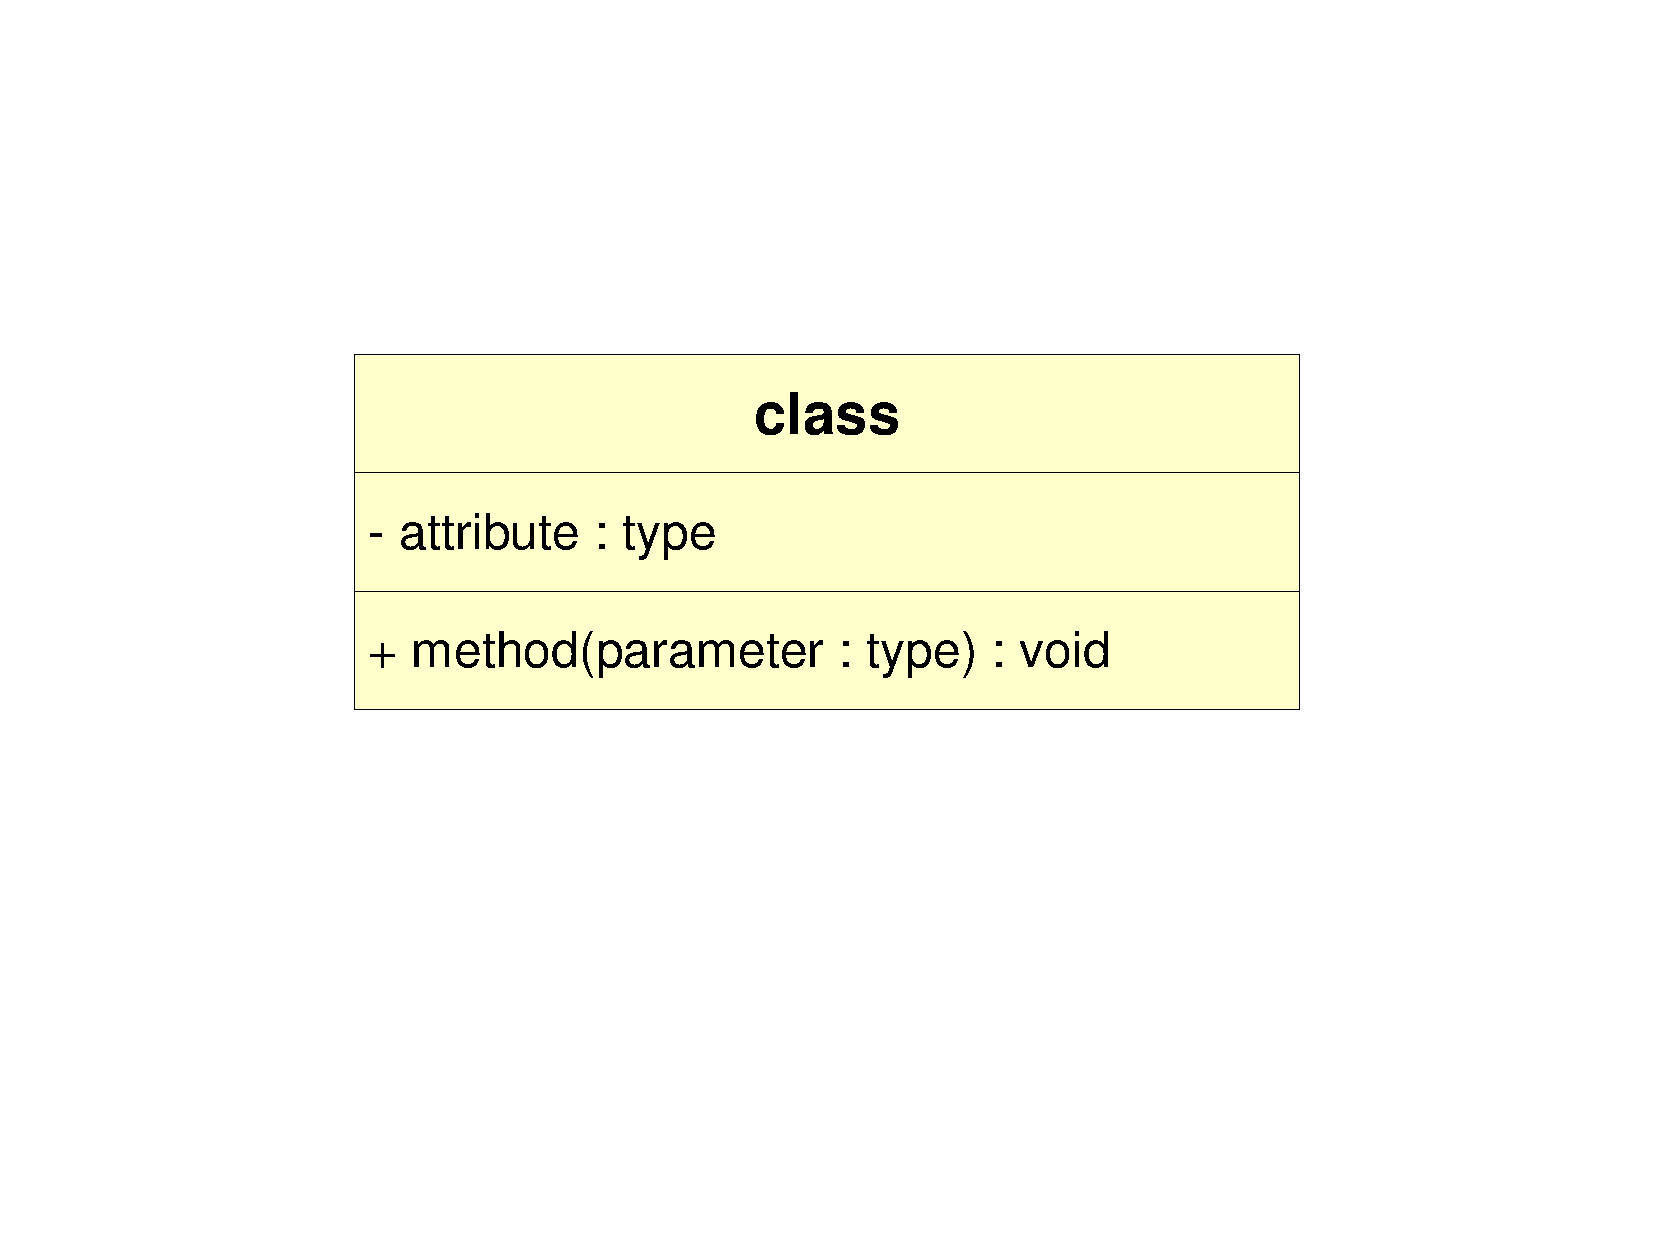
\includegraphics[scale=0.3,angle=-90]{graphic/classification.pdf}
        \caption{Classification as UML Diagram}
        \label{classification_figure}
    \end{center}
\end{figure}

While procedures and many variables in SPP are global, that is only exist once,
classes are treated as types of which many \emph{Instances} (also called
\emph{Objects}) can be created, including attributes and methods. In OOP, such
memory allocation is called \emph{Instantiation}.

Two related data types are \emph{Abstract Class} and \emph{Interface}. An
abstract class can hold attributes and (partly abstract) methods. Just like
interfaces, abstract classes cannot be instantiated. An interface is yet more
restricted in that it can only have constants but not attributes and only
declarations but not actual implementations of methods. Interfaces are commonly
used to \cite{steppan}:

\begin{itemize}
    \item[-] Realise multiple inheritance (section \ref{inheritance_heading})
    \item[-] Encapsulate components (section \ref{interface_and_implementation_heading})
    \item[-] Pool common methods (section \ref{separation_of_concerns_heading})
\end{itemize}

Specialities like \emph{Inner Classes} \cite{java} with limited scope of
validity are of minor importance to the argumentation of this document and not
further explained here.

The \emph{Bundling} of attributes and methods (state and logic) causes more
system interdependencies and complications than were predictable. It is a big
disadvantage that affects all modern object-oriented systems. \cite{heller2004}
Certainly, the bundling stems from best intentions to receive cleaner code by
keeping not only attributes but also methods in a common module, such avoiding
\emph{wild} and \emph{global} procedures. But now, modules not only have to
refer to other modules for accessing their state data; the same is needed for
accessing their logic in form of method calls.

With OOP, the number of cross-relations between modules, and inter-dependencies
between system layers may rise dramatically. In reality, state- and logic
properties are two \emph{different} things that have to be kept in different
places! Both can have a similar, hierarchical structure but each is a concept on
its own, as chapter \ref{state_and_logic_heading} will show.

%
% $RCSfile: encapsulation.tex,v $
%
% Copyright (C) 2002-2008. Christian Heller.
%
% Permission is granted to copy, distribute and/or modify this document
% under the terms of the GNU Free Documentation License, Version 1.1 or
% any later version published by the Free Software Foundation; with no
% Invariant Sections, with no Front-Cover Texts and with no Back-Cover
% Texts. A copy of the license is included in the section entitled
% "GNU Free Documentation License".
%
% http://www.cybop.net
% - Cybernetics Oriented Programming -
%
% http://www.resmedicinae.org
% - Information in Medicine -
%
% Version: $Revision: 1.1 $ $Date: 2008-08-19 20:41:06 $ $Author: christian $
% Authors: Christian Heller <christian.heller@tuxtax.de>
%

\subsubsection{Encapsulation}
\label{encapsulation_heading}
\index{Encapsulation}
\index{Access Method}
\index{Java}
\index{Information Hiding}
\index{Data Hiding}
\index{public}
\index{protected}
\index{private}
\index{Delphi}
\index{published}

One recommendation of object oriented programming is that the properties of an
object created as instance of a class be protected through special
\emph{Access Methods} (figure \ref{encapsulation_figure}). A \emph{Java} code
example can be found below. The intention is not to expose class attributes to
other classes by minimising direct access to them and such to provide some
security by preventing illegal access to an object's interna. Therefore, this
paradigm is called \emph{Encapsulation} or \emph{Information-/ Data Hiding}.
Another advantage is that if an attribute changes its name, then only one place
in the code (the access method), instead of hundreds, needs to be updated.

\begin{scriptsize}
    \begin{verbatim}
    public class example_class {
        private Type attribute;
        public void set_attribute(Type a) {
            this.attribute = a;
        }
        public Type get_attribute() {
            return this.attribute;
        }
    }
    \end{verbatim}
\end{scriptsize}

\begin{figure}[ht]
    \begin{center}
        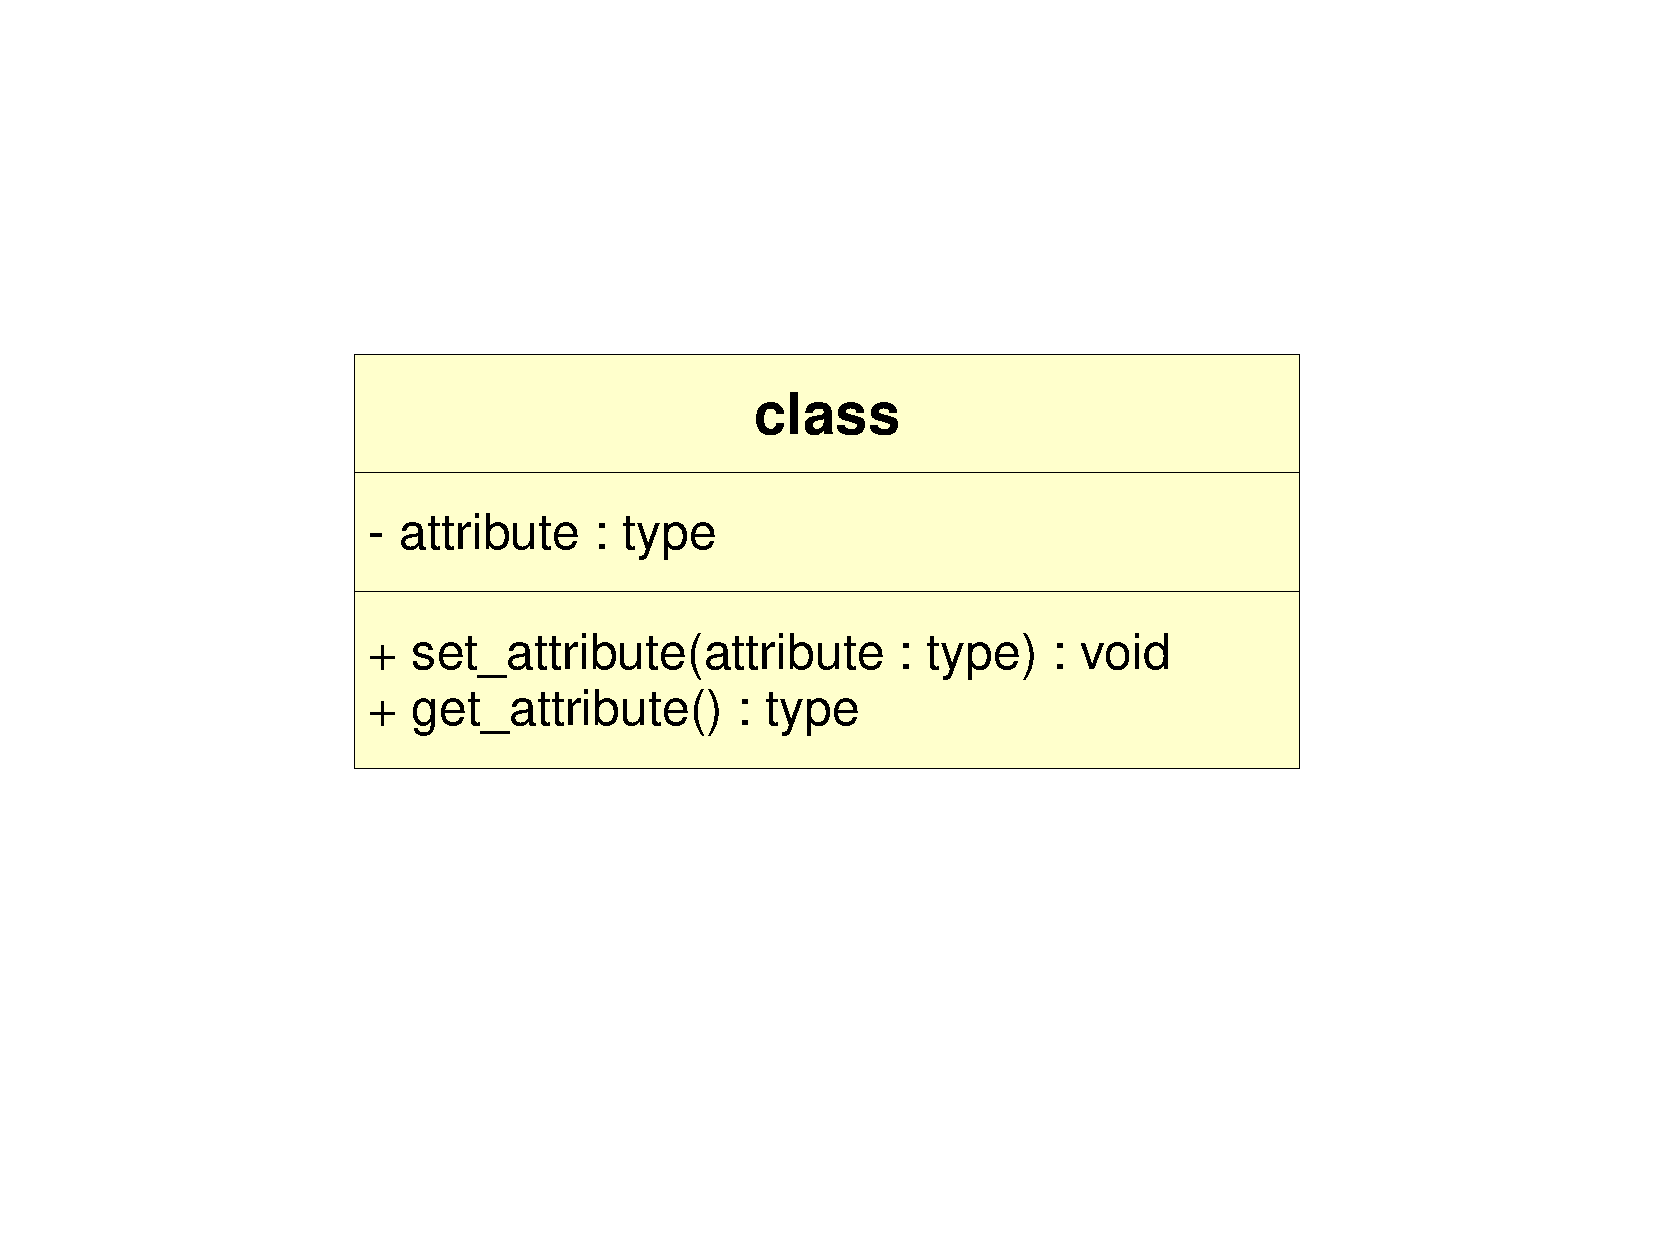
\includegraphics[scale=0.3,angle=-90]{graphic/encapsulation.pdf}
        \caption{Encapsulation as UML Diagram}
        \label{encapsulation_figure}
    \end{center}
\end{figure}

Special keywords are necessary to ensure proper encapsulation by making
attributes and methods \emph{visible} to only certain outside objects. These
keywords are: \emph{public}, \emph{protected} and \emph{private}. In the
\emph{Java} programming language \cite{java}, an additional package protection
level is applied when none of the aforementioned keywords is found. The
\emph{Delphi} language \cite{warken} knows an additional \emph{published}
keyword that makes properties visible in its object-inspector tool. Other
languages may contain further variations of access limitations.

The recommendation to encapsulate attributes produces thousands of lines of
source code whose usefulness is at least questionnable \cite{hellerbohl}. In
about 90\% of cases (practical experience of the author of this document), the
\emph{set} and \emph{get} methods consist of only one single line accessing an
attribute value which in the end is the same as accessing that attribute
directly. Sometimes, additional lines with a trigger function to update other
parts of the system are added. They get invoked whenever an attribute value of
the called object is changed by a \emph{set} method:

\begin{scriptsize}
    \begin{verbatim}
    public void set_attribute(Type a) {
        this.attribute = a;
        get_update_manager().update(this);
    }
    \end{verbatim}
\end{scriptsize}

But, as shown below, this update notification could as well be taken over by
the object that was calling the \emph{set} method:

\begin{scriptsize}
    \begin{verbatim}
    public void method() {
        example_object.set_attribute(a);
        get_update_manager().update(example_object);
    }
    \end{verbatim}
\end{scriptsize}

The argumentation that \textit{in this case a lot of redundant code would be
produced since the update function has to be implemented in every calling
object, instead of just once in the called object} does not really hold true
when looking into programming practice. The number of external objects calling
an object is mostly very well manageable. It finally seems that thousands of
\emph{set}/ \emph{get} access methods could be eliminated which would lead to a
tremendous code reduction and improved clearity.

The language introduced in chapter \ref{cybernetics_oriented_language_heading}
does not use encapsulation and the attributes (state knowledge) and methods
(logic knowledge) modelled in it are not bundled together.

%
% $RCSfile: inheritance.tex,v $
%
% Copyright (C) 2002-2008. Christian Heller.
%
% Permission is granted to copy, distribute and/or modify this document
% under the terms of the GNU Free Documentation License, Version 1.1 or
% any later version published by the Free Software Foundation; with no
% Invariant Sections, with no Front-Cover Texts and with no Back-Cover
% Texts. A copy of the license is included in the section entitled
% "GNU Free Documentation License".
%
% http://www.cybop.net
% - Cybernetics Oriented Programming -
%
% http://www.resmedicinae.org
% - Information in Medicine -
%
% Version: $Revision: 1.1 $ $Date: 2008-08-19 20:41:07 $ $Author: christian $
% Authors: Christian Heller <christian.heller@tuxtax.de>
%

\subsubsection{Inheritance}
\label{inheritance_heading}
\index{Inheritance}
\index{Superior Class}
\index{Parent Class}
\index{C++}
\index{Multiple Inheritance}
\index{Java}
\index{Single Inheritance}
\index{Interface}
\index{Application Programming Interface}
\index{API}

\emph{Inheritance} allows for code minimisation by letting classes inherit
attributes and methods from their \emph{superior} (sometimes called \emph{parent})
class (figure \ref{inheritance_figure}). Redundant code can such be avoided and
existing code can be reused. An inheriting class in \emph{Java} source code
looks like this:

\begin{scriptsize}
    \begin{verbatim}
    public class example extends super_class {
    }
    \end{verbatim}
\end{scriptsize}

\begin{figure}[ht]
    \begin{center}
        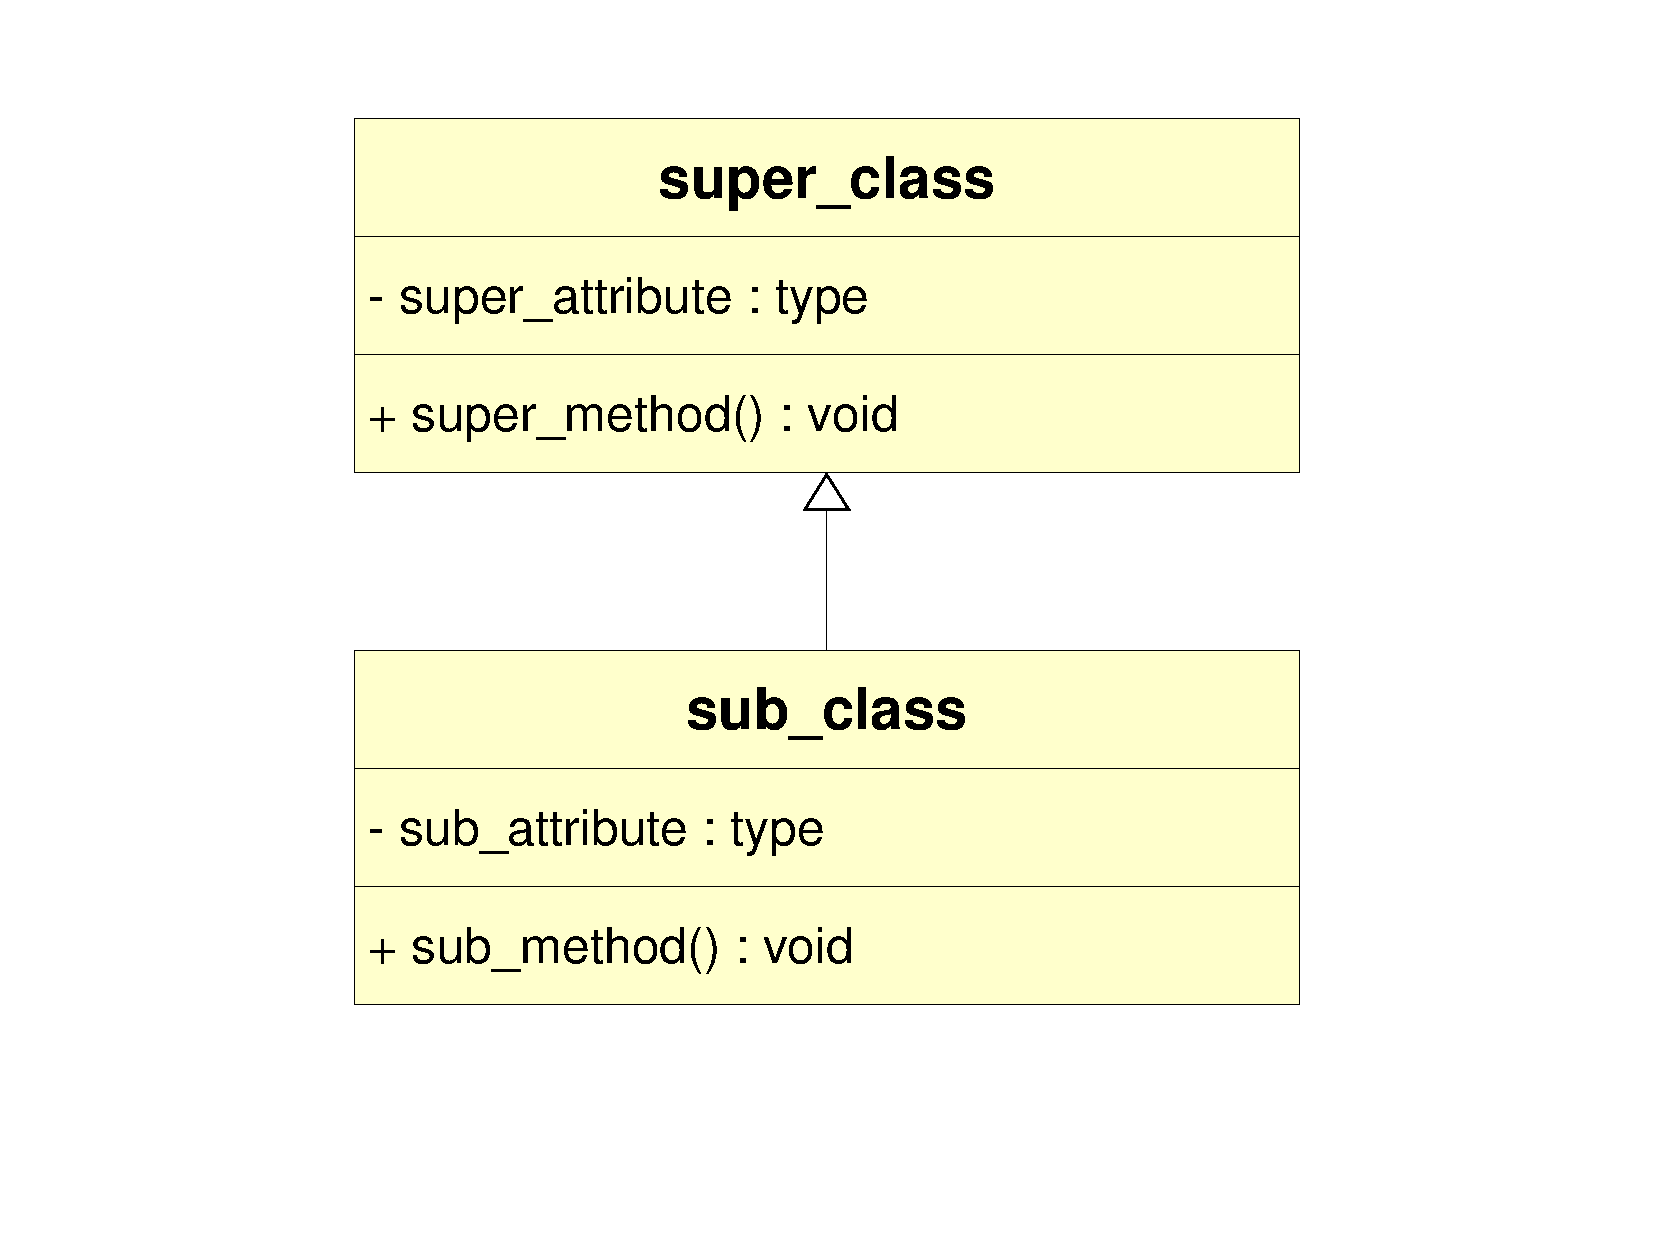
\includegraphics[scale=0.3,angle=-90]{graphic/inheritance.pdf}
        \caption{Inheritance as UML Diagram}
        \label{inheritance_figure}
    \end{center}
\end{figure}

Some object oriented programming languages (such as \emph{C++}) permit
\emph{Multiple Inheritance}. Classes written in those languages can have more
than one superior class. Other languages (such as \emph{Java}) that have
\emph{Single Inheritance} only, sometimes offer to \emph{inherit}
(\emph{realise}/ \emph{implement}) multiple interfaces. An interface forces its
subclasses to implement all methods it declares (more on this in section
\ref{interface_and_implementation_heading}) and can such provide a common
\emph{Application Programming Interface} (API) which makes classes
interchangeable and hence encourages reuse.

%
% $RCSfile: fragile_base_class.tex,v $
%
% Copyright (C) 2002-2008. Christian Heller.
%
% Permission is granted to copy, distribute and/or modify this document
% under the terms of the GNU Free Documentation License, Version 1.1 or
% any later version published by the Free Software Foundation; with no
% Invariant Sections, with no Front-Cover Texts and with no Back-Cover
% Texts. A copy of the license is included in the section entitled
% "GNU Free Documentation License".
%
% http://www.cybop.net
% - Cybernetics Oriented Programming -
%
% http://www.resmedicinae.org
% - Information in Medicine -
%
% Version: $Revision: 1.1 $ $Date: 2008-08-19 20:41:06 $ $Author: christian $
% Authors: Christian Heller <christian.heller@tuxtax.de>
%

\subsubsection{Fragile Base Class}
\label{fragile_base_class_heading}
\index{Fragile Base Class (Problem)}
\index{Implementation Inheritance}
\index{Subclass}
\index{Superclass}
\index{Class Hierarchy}
\index{Cascade of Change}
\index{Reusability}
\index{Flexibility}
\index{Cyclic Method Dependencies}
\index{Self-calling Assumptions of a Class Method}
\index{Base Class Access}
\index{Modifier Invariant Function}

Despite the possible code reduction through class inheritance, there are some
negative effects that hinder just this code reduction and reuse. John K.
Ousterhout writes in his article \cite{ousterhout1998}:

\begin{quote}
    Implementation inheritance, where one class borrows code that was written
    for another class, is a bad idea that makes software harder to manage and
    reuse. It binds the implementations of classes together so that neither
    class can be understood without the other: a subclass cannot be understood
    without knowing how the inherited methods are implemented in its superclass,
    and a superclass cannot be understood without knowing how its methods are
    inherited in subclasses. In a complex class hierarchy, no individual class
    can be understood without understanding all the other classes in the
    hierarchy. Even worse, a class cannot be separated from its hierarchy for
    reuse. Multiple inheritance makes these problems even worse. Implementation
    inheritance causes the same intertwining and brittleness that have been
    observed when goto statements are overused. As a result, object-oriented
    systems often suffer from complexity and lack of reuse.
\end{quote}

Unwanted dependencies caused simply by the usage of inheritance are called
\emph{Fragile Base Class Problem} \cite[section \emph{Layers}; p. 48]{buschmann}.
The source code changes resulting from base class manipulation are also called
\emph{Cascade of Change} \cite[Vorwort]{gruhn}. They are just the opposite of
what inheritance was actually intended to be for: \emph{Reusability}. Leonid
Mikhajlov and Emil Sekerinski \cite{mikhajlov} write:

\begin{quote}
    This problem occurs in open object-oriented systems employing code
    inheritance as an implementation reuse mechanism. System developers unaware
    of extensions to the system developed by its users may produce a seemingly
    acceptable revision of a base class which may damage its extensions.
    The fragile base class problem becomes apparent during maintenance of open
    object-oriented systems, but requires consideration during design.
\end{quote}

They identify the following \emph{Restrictions} \cite{mikhajlov} disciplining the
code inheritance mechanism, thus avoiding the \emph{Fragile Base Class Problem},
but on the cost of general \emph{Flexibility}:

\begin{itemize}
    \item[-] \emph{No cycles:} A base class revision and a modifier should not
        jointly introduce new cyclic method dependencies.
    \item[-] \emph{No revision self-calling assumptions:} Revision class methods
        should not make any additional assumptions about the behaviour of the
        other methods of itself. Only the behaviour described in the base class
        may be taken into consideration.
    \item[-] \emph{No base class down-calling assumptions:} Methods of a modifier
        should disregard the fact that base class self-calls can get redirected
        to the modifier itself. In this case bodies of the corresponding methods
        in the base class should be considered instead, as if there were no
        dynamic binding.
    \item[-] \emph{No direct access to base class state:} An extension class
        may not access the state of its base class directly, but only through
        calling base class methods.
    \item[-] \emph{No modifier invariant function:} A modifier should not bind
        values of its instance variables with values of the intended base class
        instance variables to generate an invariant.
\end{itemize}

In order to remain highly flexible and to avoid the fragile base class problem,
the language described in chapter \ref{cybernetics_oriented_language_heading}
does not use inheritance, although it could be extended to do so. In this case,
of course, its interpreter (chapter \ref{cybernetics_oriented_interpreter_heading})
would have to be adapted as well.

%
% $RCSfile: polymorphism.tex,v $
%
% Copyright (C) 2002-2008. Christian Heller.
%
% Permission is granted to copy, distribute and/or modify this document
% under the terms of the GNU Free Documentation License, Version 1.1 or
% any later version published by the Free Software Foundation; with no
% Invariant Sections, with no Front-Cover Texts and with no Back-Cover
% Texts. A copy of the license is included in the section entitled
% "GNU Free Documentation License".
%
% http://www.cybop.net
% - Cybernetics Oriented Programming -
%
% http://www.resmedicinae.org
% - Information in Medicine -
%
% Version: $Revision: 1.1 $ $Date: 2008-08-19 20:41:08 $ $Author: christian $
% Authors: Christian Heller <christian.heller@tuxtax.de>
%

\subsubsection{Polymorphism}
\label{polymorphism_heading}
\index{Polymorphism}
\index{Method Overloading}
\index{Method Overriding}
\index{Super Class}
\index{Sub Class}
\index{super}

Another object oriented feature that comes with inheritance is
\emph{Polymorphism}. It allows methods to be \emph{overloaded} (sometimes
called \emph{overridden}). That is, on two objects created from different
classes inheriting from each other, the right equally named method will be
called by the language interpreter program (figure \ref{polymorphism_figure}),
which leads to different behaviour depending on the current object context.
Following is a \emph{Java} code example overloading a method to gain
polymorphic behaviour:

\begin{scriptsize}
    \begin{verbatim}
    public class super_class {
        public void method() {
            do_something();
        }
    }
    public class sub_class extends super_class {
        public void method() {
            do_something_else();
        }
    }
    \end{verbatim}
\end{scriptsize}

\begin{figure}[ht]
    \begin{center}
        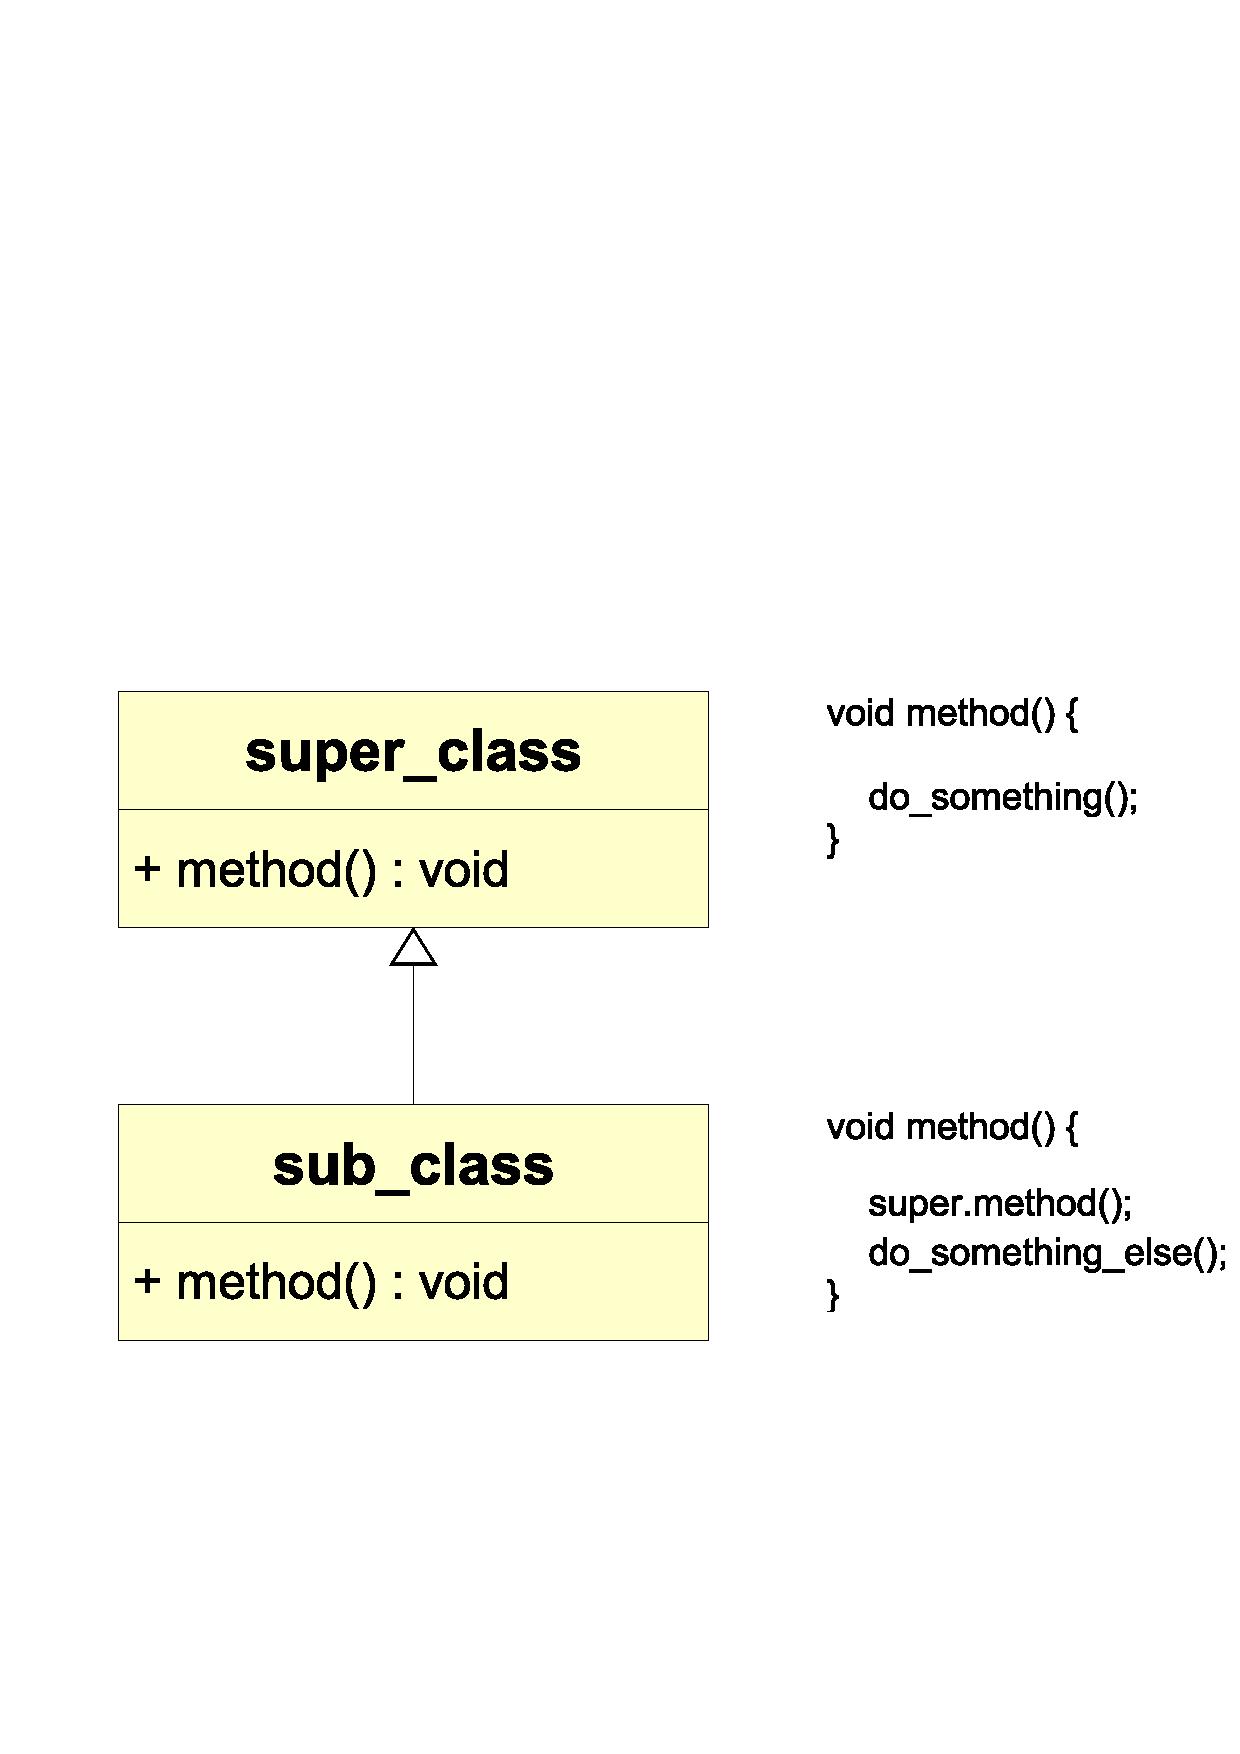
\includegraphics[scale=0.3,angle=-90]{graphic/polymorphism.pdf}
        \caption{Polymorphism as UML Diagram}
        \label{polymorphism_figure}
    \end{center}
\end{figure}

If objects instantiated from a sub class want to make use of the functionality
contained in the super class' equally named method, the sub class' method needs
to call the super class' method explicitly using the keyword \emph{super}:

\begin{scriptsize}
    \begin{verbatim}
    public class sub_class extends super_class {
        public void method() {
            super.method();
            do_something_else();
        }
    }
    \end{verbatim}
\end{scriptsize}

%
% $RCSfile: container.tex,v $
%
% Copyright (C) 2002-2008. Christian Heller.
%
% Permission is granted to copy, distribute and/or modify this document
% under the terms of the GNU Free Documentation License, Version 1.1 or
% any later version published by the Free Software Foundation; with no
% Invariant Sections, with no Front-Cover Texts and with no Back-Cover
% Texts. A copy of the license is included in the section entitled
% "GNU Free Documentation License".
%
% http://www.cybop.net
% - Cybernetics Oriented Programming -
%
% http://www.resmedicinae.org
% - Information in Medicine -
%
% Version: $Revision: 1.1 $ $Date: 2008-08-19 20:41:06 $ $Author: christian $
% Authors: Christian Heller <christian.heller@tuxtax.de>
%

\subsubsection{Container}
\label{container_heading}
\index{Container}
\index{Primitive Type}
\index{Java Container Framework}
\index{Collection}
\index{Map}
\index{Tree}
\index{Standard Template Library}
\index{STL}
\index{Sequence}
\index{Associative Container}

An object that got created through instantiating a class represents an
allocated area in a computer's memory which needs to be referenced in order to
be able to work with it, and to finally destroy it. The size of that area may
change \emph{dynamically}, depending on how the properties of the object are
manipulated. Primitive types like \emph{integer} or \emph{double} also reserve
memory space, only that the size of that space is \emph{not} dynamic; it is
pre-defined by the programming language, for each type. All
\emph{Structured- and Procedural Programming} (SPP) languages and some
\emph{Object Oriented Programming} (OOP) languages, like Java, offer standard
primitive types.

\begin{figure}[ht]
    \begin{center}
        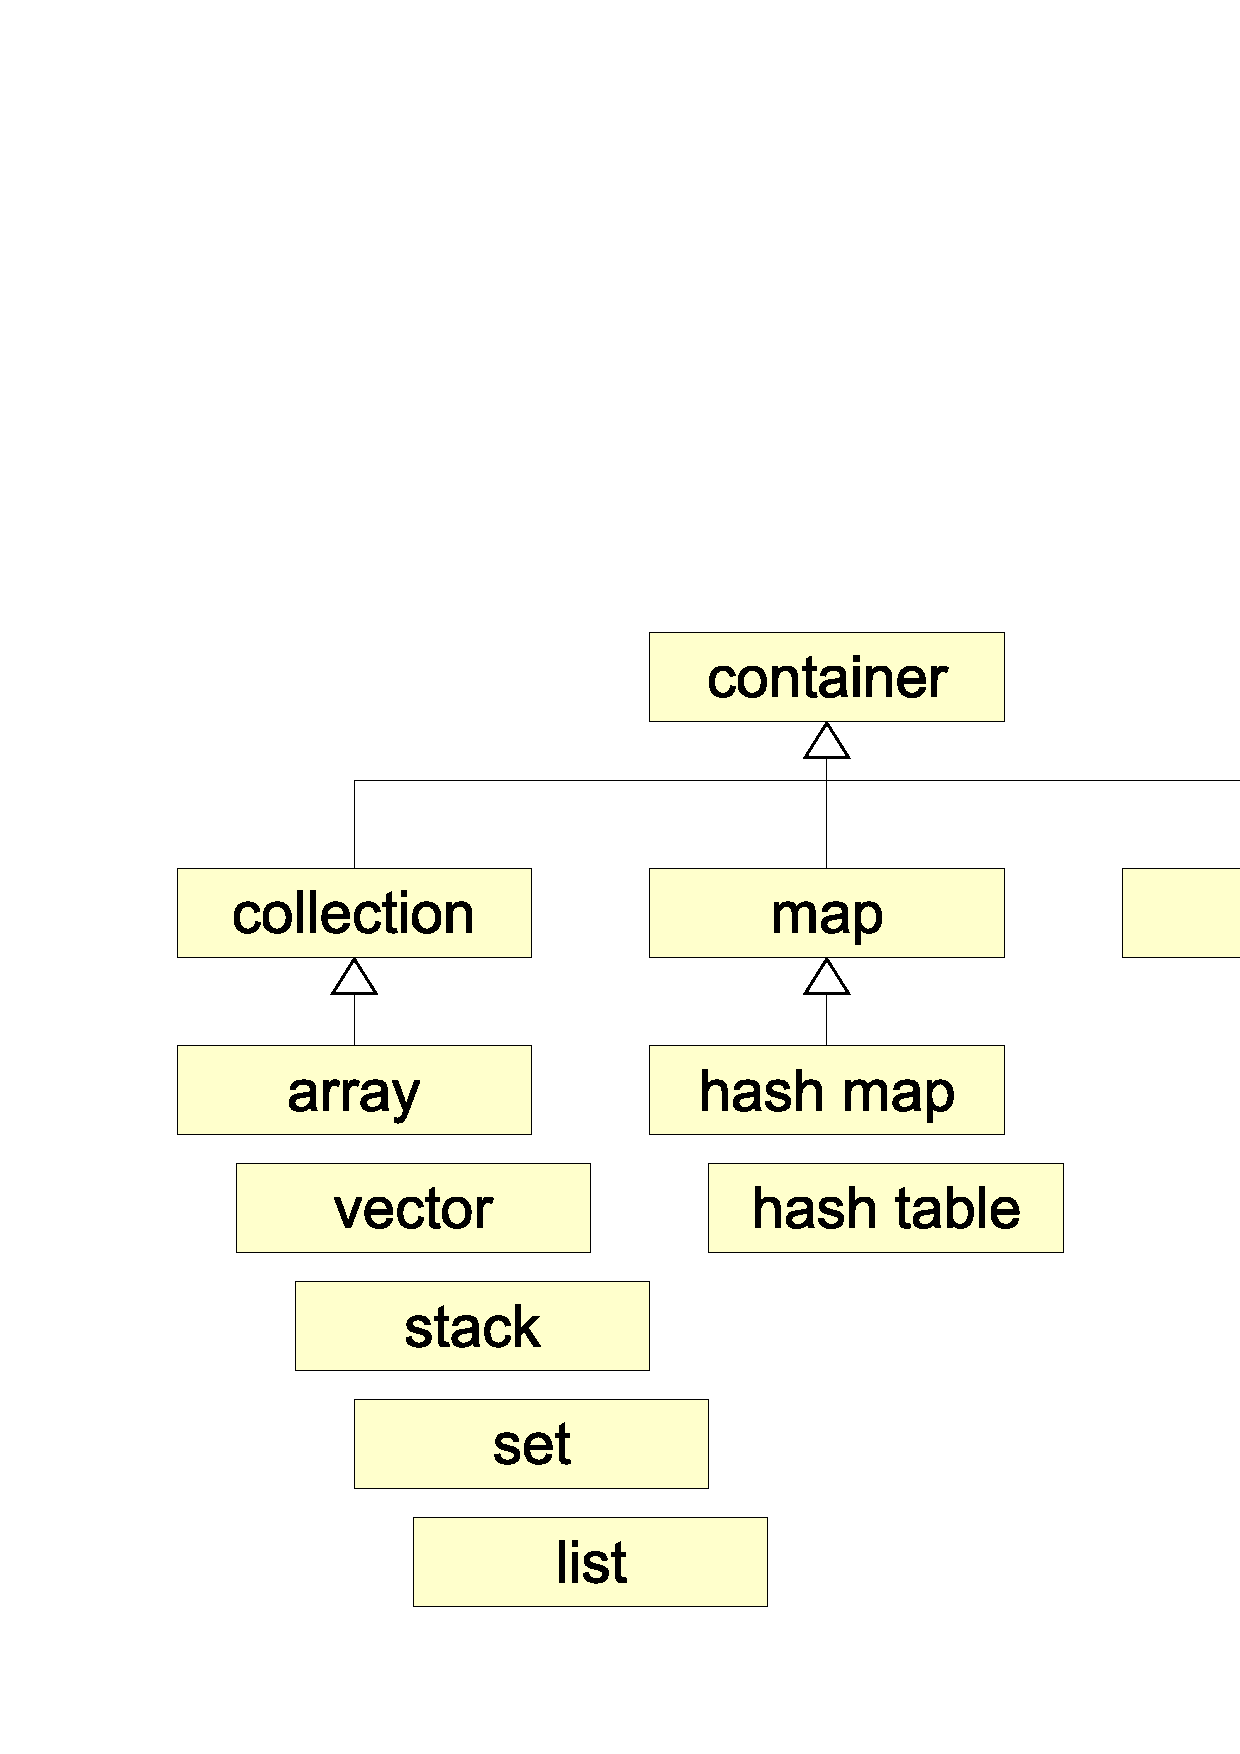
\includegraphics[scale=0.3,angle=-90]{graphic/container.pdf}
        \caption{Java Container Framework Systematics}
        \label{container_figure}
    \end{center}
\end{figure}

One way to store references to more than one dynamic element in memory, or
primitive data, is a \emph{Container}. Modern programming languages offer many
different kinds of containers. Figure \ref{container_figure} shows a
systematics of the Java container framework \cite{java}, as example, which gets
briefly introduced in the following paragraphs. Its main categories of
systematisation are \emph{Collection}, \emph{Map} and \emph{Tree}.

A similar library of container classes, algorithms and iterators exists for the
C++ programming language. It is called \emph{Standard Template Library} (STL)
\cite{stl} and it talks of \emph{Sequence} and \emph{Associative Container},
where Java says \emph{Collection} and \emph{Map}.

%
% $RCSfile: collection.tex,v $
%
% Copyright (C) 2002-2008. Christian Heller.
%
% Permission is granted to copy, distribute and/or modify this document
% under the terms of the GNU Free Documentation License, Version 1.1 or
% any later version published by the Free Software Foundation; with no
% Invariant Sections, with no Front-Cover Texts and with no Back-Cover
% Texts. A copy of the license is included in the section entitled
% "GNU Free Documentation License".
%
% http://www.cybop.net
% - Cybernetics Oriented Programming -
%
% http://www.resmedicinae.org
% - Information in Medicine -
%
% Version: $Revision: 1.1 $ $Date: 2008-08-19 20:41:05 $ $Author: christian $
% Authors: Christian Heller <christian.heller@tuxtax.de>
%

\paragraph{Collection}
\label{collection_heading}
\index{Collection}
\index{Array}
\index{Allocated Area}
\index{Random Access Memory}
\index{RAM}
\index{Vector}
\index{Stack}
\index{Last-In-First-Out}
\index{LIFO}
\index{Set}
\index{List}
\index{Duplicate Element}
\index{Ordered Collection}
\index{Sequence}
\index{Enumeration}
\index{nextElement Method}
\index{Java Development Kit}
\index{JDK}
\index{Iterator}

The \emph{Array} is the most basic form of a container. It represents an allocated
area in the computer's \emph{Random Access Memory} (RAM). A \emph{Vector}
implements a dynamically growable array of objects. The \emph{Stack} class extends
the vector class and represents a \emph{Last-In-First-Out} (LIFO) stack of objects.
A collection that contains no duplicate elements is called a \emph{Set}. Unlike
sets, \emph{Lists} typically allow duplicate elements. Synonyms for list are
\emph{Ordered Collection} and \emph{Sequence}.

Objects that can generate a series of elements, one at a time, implement the
\emph{Enumeration} interface. Successive calls to the \emph{nextElement} method
return successive elements of such a series. In recent releases of the
\emph{Java Development Kit} (JDK) \cite{java}, \emph{Iterator} takes the place
of enumeration, in the collections framework. An iterator over a collection
differs from an enumeration in that it allows the caller to remove elements,
with well-defined semantics, from the underlying collection during an iteration.

%
% $RCSfile: map.tex,v $
%
% Copyright (C) 2002-2008. Christian Heller.
%
% Permission is granted to copy, distribute and/or modify this document
% under the terms of the GNU Free Documentation License, Version 1.1 or
% any later version published by the Free Software Foundation; with no
% Invariant Sections, with no Front-Cover Texts and with no Back-Cover
% Texts. A copy of the license is included in the section entitled
% "GNU Free Documentation License".
%
% http://www.cybop.net
% - Cybernetics Oriented Programming -
%
% http://www.resmedicinae.org
% - Information in Medicine -
%
% Version: $Revision: 1.1 $ $Date: 2008-08-19 20:41:07 $ $Author: christian $
% Authors: Christian Heller <christian.heller@tuxtax.de>
%

\paragraph{Map}
\label{map_heading}
\index{Map}
\index{Dictionary}
\index{Table}
\index{Key-Value-Pair}
\index{Duplicate Key}
\index{Hash Map}
\index{Hash Table}
\index{Null Value}
\index{Null Key}

A \emph{Map} (also called \emph{Dictionary} or \emph{Table}) is an object that
maps \emph{Keys} to \emph{Values}. It cannot contain duplicate keys; each key
can map to at most one value. Java offers two kinds of a map: \emph{Hash Map}
and \emph{Hash Table}. The former is roughly equivalent to the latter, except
that it permits null values and the null key \cite{java, gumbel}.

%
% $RCSfile: tree.tex,v $
%
% Copyright (C) 2002-2008. Christian Heller.
%
% Permission is granted to copy, distribute and/or modify this document
% under the terms of the GNU Free Documentation License, Version 1.1 or
% any later version published by the Free Software Foundation; with no
% Invariant Sections, with no Front-Cover Texts and with no Back-Cover
% Texts. A copy of the license is included in the section entitled
% "GNU Free Documentation License".
%
% http://www.cybop.net
% - Cybernetics Oriented Programming -
%
% http://www.resmedicinae.org
% - Information in Medicine -
%
% Version: $Revision: 1.1 $ $Date: 2008-08-19 20:41:09 $ $Author: christian $
% Authors: Christian Heller <christian.heller@tuxtax.de>
%

\paragraph{Tree}
\label{tree_heading}
\index{Tree}
\index{Tree Node}
\index{Leaf Tree Node}
\index{Branch Tree Node}
\index{Root Tree Node}

A \emph{Tree}, or more exact \emph{Tree Node}, is a further kind of container.
Many tree nodes, in hierarchical order, may form a tree. A tree node may
represent a \emph{Leaf} with no children or a \emph{Branch} with one or more
children. The top-most tree node is usually called \emph{Root}.


%
% $RCSfile: falsifying_polymorphism.tex,v $
%
% Copyright (C) 2002-2008. Christian Heller.
%
% Permission is granted to copy, distribute and/or modify this document
% under the terms of the GNU Free Documentation License, Version 1.1 or
% any later version published by the Free Software Foundation; with no
% Invariant Sections, with no Front-Cover Texts and with no Back-Cover
% Texts. A copy of the license is included in the section entitled
% "GNU Free Documentation License".
%
% http://www.cybop.net
% - Cybernetics Oriented Programming -
%
% http://www.resmedicinae.org
% - Information in Medicine -
%
% Version: $Revision: 1.1 $ $Date: 2008-08-19 20:41:06 $ $Author: christian $
% Authors: Christian Heller <christian.heller@tuxtax.de>
%

\subsubsection{Falsifying Polymorphism}
\label{falsifying_polymorphism_heading}
\index{Falsifying Polymorphism}
\index{Container Inheritance}
\index{Hashtable}
\index{Copy Constructor}

Problems can occur when inheriting containers. This is now demonstrated on a Java
example adopted from \cite{javaiaq}.

\begin{figure}[ht]
    \begin{center}
        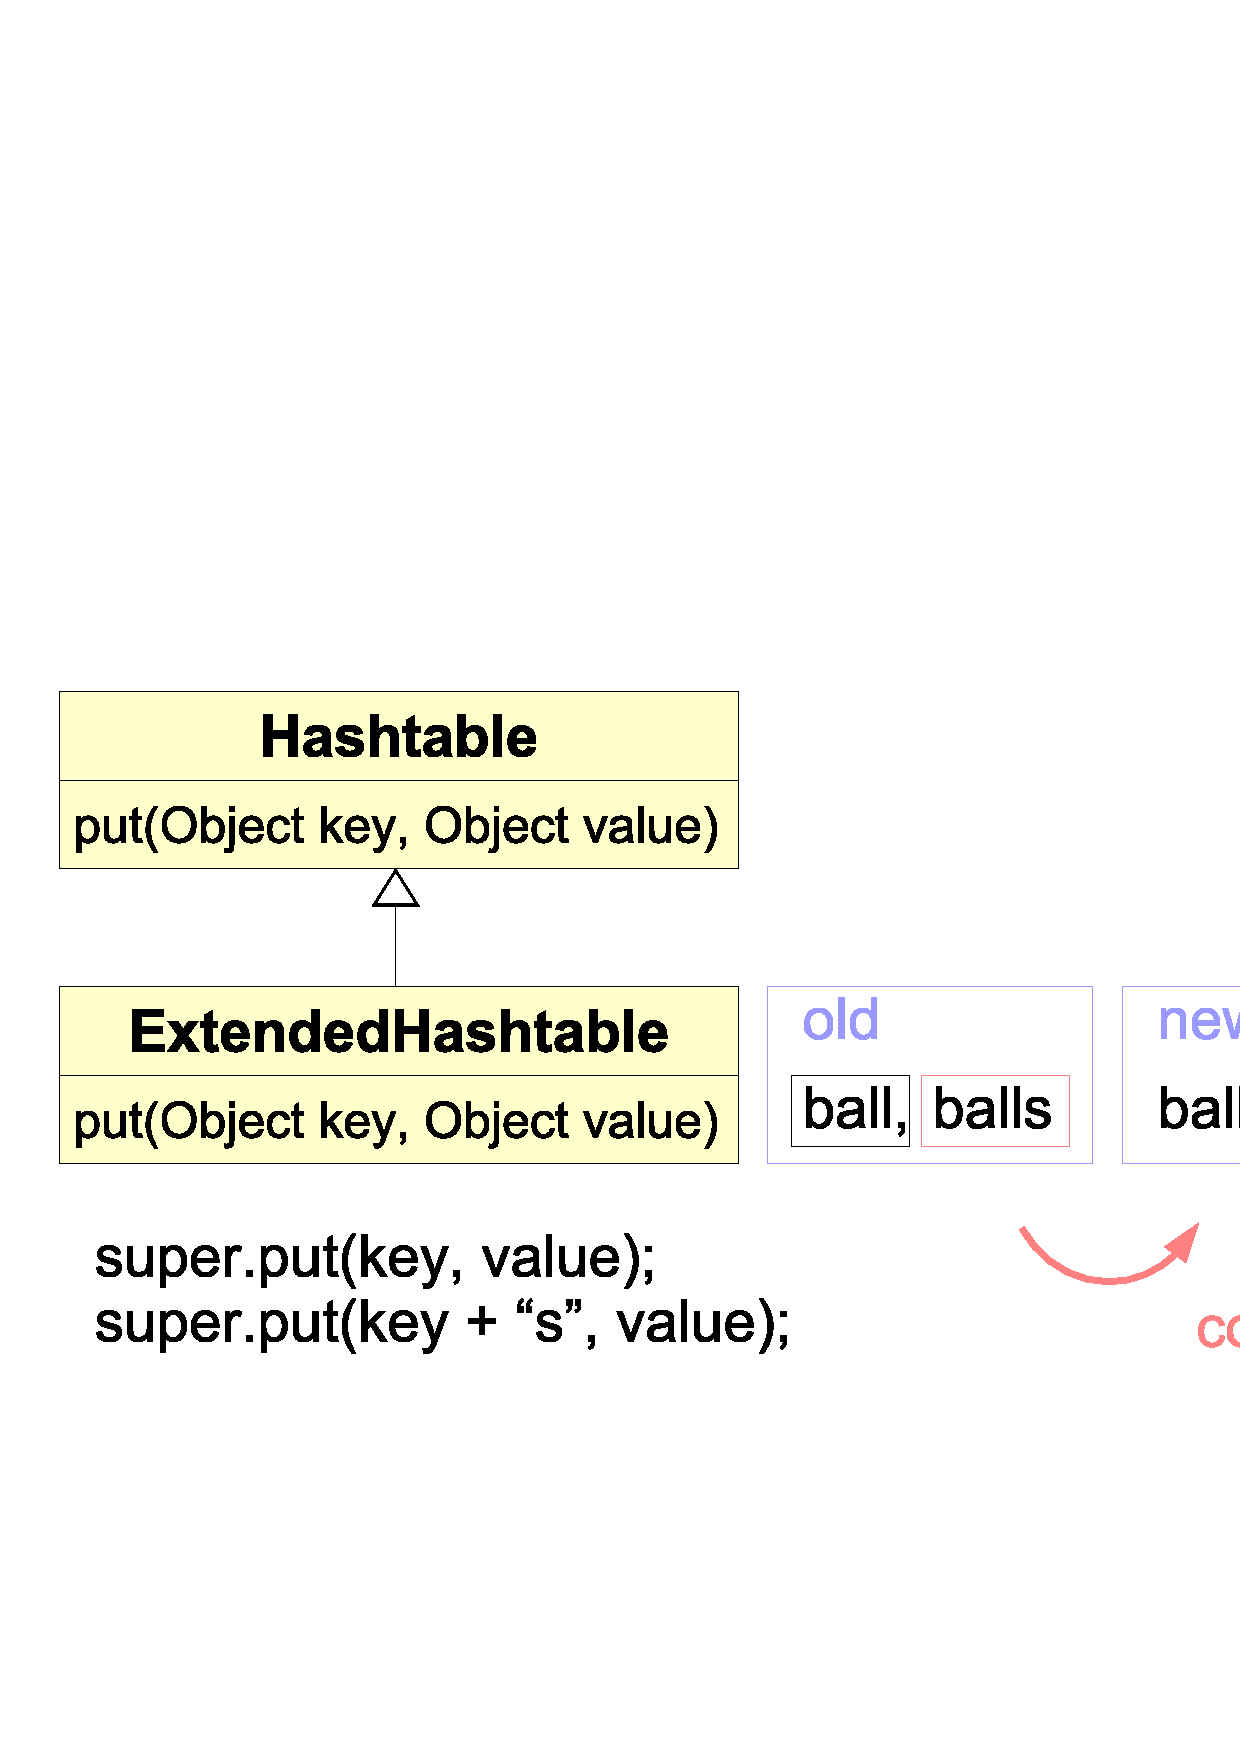
\includegraphics[scale=0.3,angle=-90]{graphic/falsifying.pdf}
        \caption{Falsified Contents with Container Inheritance}
        \label{falsifying_figure}
    \end{center}
\end{figure}

A class \emph{ExtendedHashtable} extends the standard container \emph{Hashtable}
(figure \ref{falsifying_figure}). The \emph{ExtendedHashtable} overrides the
\emph{put} method and lets it do two calls to the \emph{put} method of the
superior class \emph{Hashtable}, the second of these calls adding the letter
\emph{s} to the key.

A first object of type \emph{ExtendedHashtable} gets filled by calling the
\emph{put} method which adds two identical element values with the two different
keys \emph{ball} and \emph{balls} to the container. When the container is full,
a new one with extended size gets created and all values of the old have to be
copied into the new container, which is again of type \emph{ExtendedHashtable}.

If the \emph{put} method is now used to accomplish this, a falsified container
with more elements than the original one will be retrieved. The copying of the
first element \emph{ball} results in two elements \emph{ball} and \emph{balls},
placed in the new container. The copying of the second element \emph{balls} adds
two further elements \emph{balls} and \emph{ballss}, whereby the \emph{balls}
key stemming from the copying of the first element gets overwritten.

This example demonstrates only the principle of how the automatic size
extension of inherited container objects with element copying using
container-owned methods can incorrectly modify the container contents. The Java
language's \emph{Hashtable} class uses a slightly different mechanism, handing
over the hashtable object as parameter of a copy constructor which internally
calls a \emph{putAll} method which finally calls the \emph{put} method. Other
OOP languages may use different mechanisms. Of course, there are workarounds to
avoid the described troubles. But as a matter of fact, container inheritance
may -- due to polymorphism -- cause unpredictable behaviour leading to
\emph{falsified} container contents.

The language and interpreter introduced in chapters
\ref{cybernetics_oriented_language_heading} and
\ref{cybernetics_oriented_interpreter_heading} base on just one container
structure for knowledge representation, that covers many of the traditional
forms of containers.

%
% $RCSfile: conclusion.tex,v $
%
% Copyright (C) 2002-2008. Christian Heller.
%
% Permission is granted to copy, distribute and/or modify this document
% under the terms of the GNU Free Documentation License, Version 1.1 or
% any later version published by the Free Software Foundation; with no
% Invariant Sections, with no Front-Cover Texts and with no Back-Cover
% Texts. A copy of the license is included in the section entitled
% "GNU Free Documentation License".
%
% http://www.cybop.net
% - Cybernetics Oriented Programming -
%
% http://www.resmedicinae.org
% - Information in Medicine -
%
% Version: $Revision: 1.1 $ $Date: 2008-08-19 20:41:06 $ $Author: christian $
% Authors: Christian Heller <christian.heller@tuxtax.de>
%

\subsubsection{Conclusion}
\label{conclusion_heading}
\index{OOP Innovations}
\index{Object Oriented Programming}
\index{OOP}
\index{Structured and Procedural Programming}
\index{SPP}

As could be seen in the previous sections, OOP contributed many new concepts
to software design, thus trying to improve SPP. Most importantly, SPP data
structures (struct, record) got extended towards the \emph{Class} which does
not only hold data (attributes), but also operations (methods). This brought
with the concept of \emph{Encapsulation}, which permits only special methods of
an \emph{Object} (class instance) to access the data (properties) of that same
object. The next innovation was \emph{Inheritance}, which allows a class to
reuse the attributes and methods of its super class(es). Finally, inheritance
was used to introduce the concept of \emph{Polymorphism}, which lets objects
react differently, depending on the class they were instantiated with.

All of these concepts were true innovations as compared with traditional SPP
techniques. However, they have their own drawbacks: growth of the number of
dependencies within a system (links between classes), caused by the bundling of
attributes and methods; fragile base class problem; falsified container
contents with container inheritance. This work will not just revise these
concepts, but turn them upside down. Data (attributes) and operations/
algorithms (methods) are not bundled any longer; the resolution of inheritance
relationships at runtime gets eliminated and with it polymorphism; container
inheritance is not necessary any longer, since only one global container
structure (knowledge container) is used in a system. More on that in part
\ref{contribution_heading} of this work.


